% ============================================================
%  Simulazione SU2 Aeroacustica — Jet Impingente su Chip
%  Documento tecnico per Sebastiano / Huawei Research Finland
%  Aprile 2026 — Prof. A. Bottaro, Università di Genova
% ============================================================
\documentclass[11pt,a4paper]{article}

% ---------- encoding & lingua ----------
\usepackage[utf8]{inputenc}
\usepackage[T1]{fontenc}
\usepackage{lmodern}
\usepackage[italian]{babel}

% ---------- layout ----------
\usepackage[top=2.5cm,bottom=2.5cm,left=2.5cm,right=2.5cm]{geometry}
\usepackage[protrusion=true,expansion=false]{microtype}
\setlength{\headheight}{14pt}
\usepackage{parskip}
\setlength{\parskip}{0.5\baselineskip}
\setlength{\parindent}{0pt}

% ---------- matematica ----------
\usepackage{amsmath}
\usepackage{amssymb}
\usepackage{mathtools}

% ---------- grafica ----------
\usepackage{graphicx}
\graphicspath{{figs/}}
\usepackage{float}
\usepackage{caption}
\captionsetup{font=small,labelfont=bf,skip=6pt}
\usepackage{subcaption}

% ---------- tabelle ----------
\usepackage{booktabs}
\usepackage{tabularx}
\usepackage{array}
\usepackage{longtable}
\usepackage{multirow}

% ---------- colori ----------
\usepackage[table]{xcolor}
\definecolor{huaweiblue}{HTML}{1A365D}
\definecolor{midblue}{HTML}{2C5282}
\definecolor{lightblue}{HTML}{EBF4FF}
\definecolor{tablehead}{HTML}{D6E4F7}
\definecolor{codegray}{HTML}{444444}
\definecolor{codebg}{HTML}{F5F5F5}
\definecolor{keywordcolor}{HTML}{1A365D}
\definecolor{valuecolor}{HTML}{2C5282}
\definecolor{commentcolor}{HTML}{6A737D}

% ---------- listings ----------
\usepackage{listings}
\lstdefinestyle{SU2cfg}{%
  backgroundcolor=\color{codebg},
  basicstyle=\ttfamily\small,
  breaklines=true,
  breakatwhitespace=false,
  columns=fullflexible,
  keepspaces=true,
  frame=single,
  framerule=0.4pt,
  rulecolor=\color{midblue!40},
  tabsize=2,
  showstringspaces=false,
  commentstyle=\color{commentcolor}\itshape,
  morecomment=[l]{\%},
  keywordstyle=\color{keywordcolor}\bfseries,
  stringstyle=\color{valuecolor},
  morekeywords={SOLVER,KIND_TURB_MODEL,KIND_SGS_MODEL,MATH_PROBLEM,
    RESTART_SOL,INC_DENSITY_MODEL,INC_DENSITY_INIT,INC_VELOCITY_INIT,
    INC_NONDIM,VISCOSITY_MODEL,MU_CONSTANT,TIME_DOMAIN,TIME_MARCHING,
    TIME_STEP,MAX_TIME,INNER_ITER,CONV_RESIDUAL_MINVAL,NUM_METHOD_GRAD,
    CFL_NUMBER,MUSCL_FLOW,SLOPE_LIMITER_FLOW,CONV_NUM_METHOD_FLOW,
    TIME_DISCRE_FLOW,JST_SENSOR_COEFF,MARKER_INLET,MARKER_OUTLET,
    MARKER_HEATFLUX,ACOUSTIC_ANALOGY,MARKER_ACOUSTIC,OBSERVER_LOCATIONS,
    FREQ_LIMIT_FWH,OUTPUT_WRT_FREQ,VOLUME_OUTPUT,SCREEN_OUTPUT,
    HISTORY_OUTPUT,PARTITION_FILE,ITER,CFL_ADAPT,CFL_ADAPT_PARAM,
    CONV_NUM_METHOD_FLOW},
  literate={=}{{\textcolor{codegray}{=}}}1
}
\lstset{style=SU2cfg}

% ---------- hyperref ----------
\usepackage{hyperref}
\hypersetup{%
  colorlinks=true,
  linkcolor=huaweiblue,
  citecolor=midblue!70!black,
  urlcolor=midblue,
  pdftitle={Simulazione SU2 Aeroacustica Jet Impingente su Chip},
  pdfauthor={Prof. A. Bottaro — Università di Genova},
  bookmarksnumbered=true
}

% ---------- section styling ----------
\usepackage{titlesec}
\titleformat{\section}{\large\bfseries\color{huaweiblue}}{\thesection}{1em}{}[\vspace{-4pt}\color{midblue}\rule{\linewidth}{0.4pt}\vspace{2pt}]
\titleformat{\subsection}{\normalsize\bfseries\color{midblue}}{\thesubsection}{1em}{}
\titleformat{\subsubsection}{\normalsize\bfseries\color{midblue!70!black}}{\thesubsubsection}{1em}{}

% ---------- comandi custom ----------
\newcommand{\ttcfg}[1]{\texttt{\color{codegray}#1}}
\newcommand{\kw}[1]{\texttt{\color{keywordcolor}\bfseries #1}}
\newcommand{\Djet}{D_{\mathrm{jet}}}
\newcommand{\Dcam}{D_{\mathrm{cam}}}
\newcommand{\Hcam}{H_{\mathrm{cam}}}
\newcommand{\Rey}{\mathrm{Re}}
\newcommand{\Ma}{\mathrm{Ma}}
\newcommand{\Str}{\mathrm{St}}
\newcommand{\mum}{\,\mu\mathrm{m}}
\newcommand{\mus}{\,\mu\mathrm{s}}
\newcommand{\ms}{\,\mathrm{ms}}
\newcommand{\tFT}{t_{\mathrm{FT}}}

% ---------- header/footer ----------
\usepackage{fancyhdr}
\pagestyle{fancy}
\fancyhf{}
\fancyhead[L]{\small\color{midblue}\textit{Simulazione SU2 — Jet Impingente su Chip}}
\fancyhead[R]{\small\color{midblue}\textit{Huawei Research Finland / UniGe, Aprile 2026}}
\fancyfoot[C]{\small\thepage}
\renewcommand{\headrulewidth}{0.4pt}
\renewcommand{\headrule}{\color{midblue!40}\hrule width\headwidth height\headrulewidth}

% ============================================================
\begin{document}
% ============================================================

% -------- FRONTESPIZIO --------
\begin{titlepage}
  \centering
  \vspace*{1.5cm}

  {\color{huaweiblue}\rule{\linewidth}{1.5pt}}
  \vspace{0.6cm}

  {\LARGE\bfseries\color{huaweiblue}
    Simulazione Aeroacustica CFD \\[0.3cm]
    di un Getto Impingente su Chip \\[0.3cm]
    tramite SU2
  }

  \vspace{0.4cm}
  {\color{midblue}\rule{\linewidth}{0.8pt}}

  \vspace{0.8cm}
  {\large\itshape
    Setup completo: geometria, pipeline LES, progressione mesh, \\
    analisi hardware/costi e roadmap temporale
  }

  \vspace{1.2cm}
  \begin{tabular}{rl}
    \textbf{Committente:}   & Huawei Research Center Finland \\
    \textbf{Referente:}     & Sebastiano \\
    \textbf{Consulente:}    & Prof.\ A.~Bottaro, Università di Genova \\
    \textbf{Solver:}        & SU2 v8 (open source, multiphysics) \\
    \textbf{Data:}          & Aprile 2026 \\
    \textbf{Versione:}      & 1.0 — Documento Tecnico Preliminare \\
  \end{tabular}

  \vspace{1.5cm}
  \begin{center}
    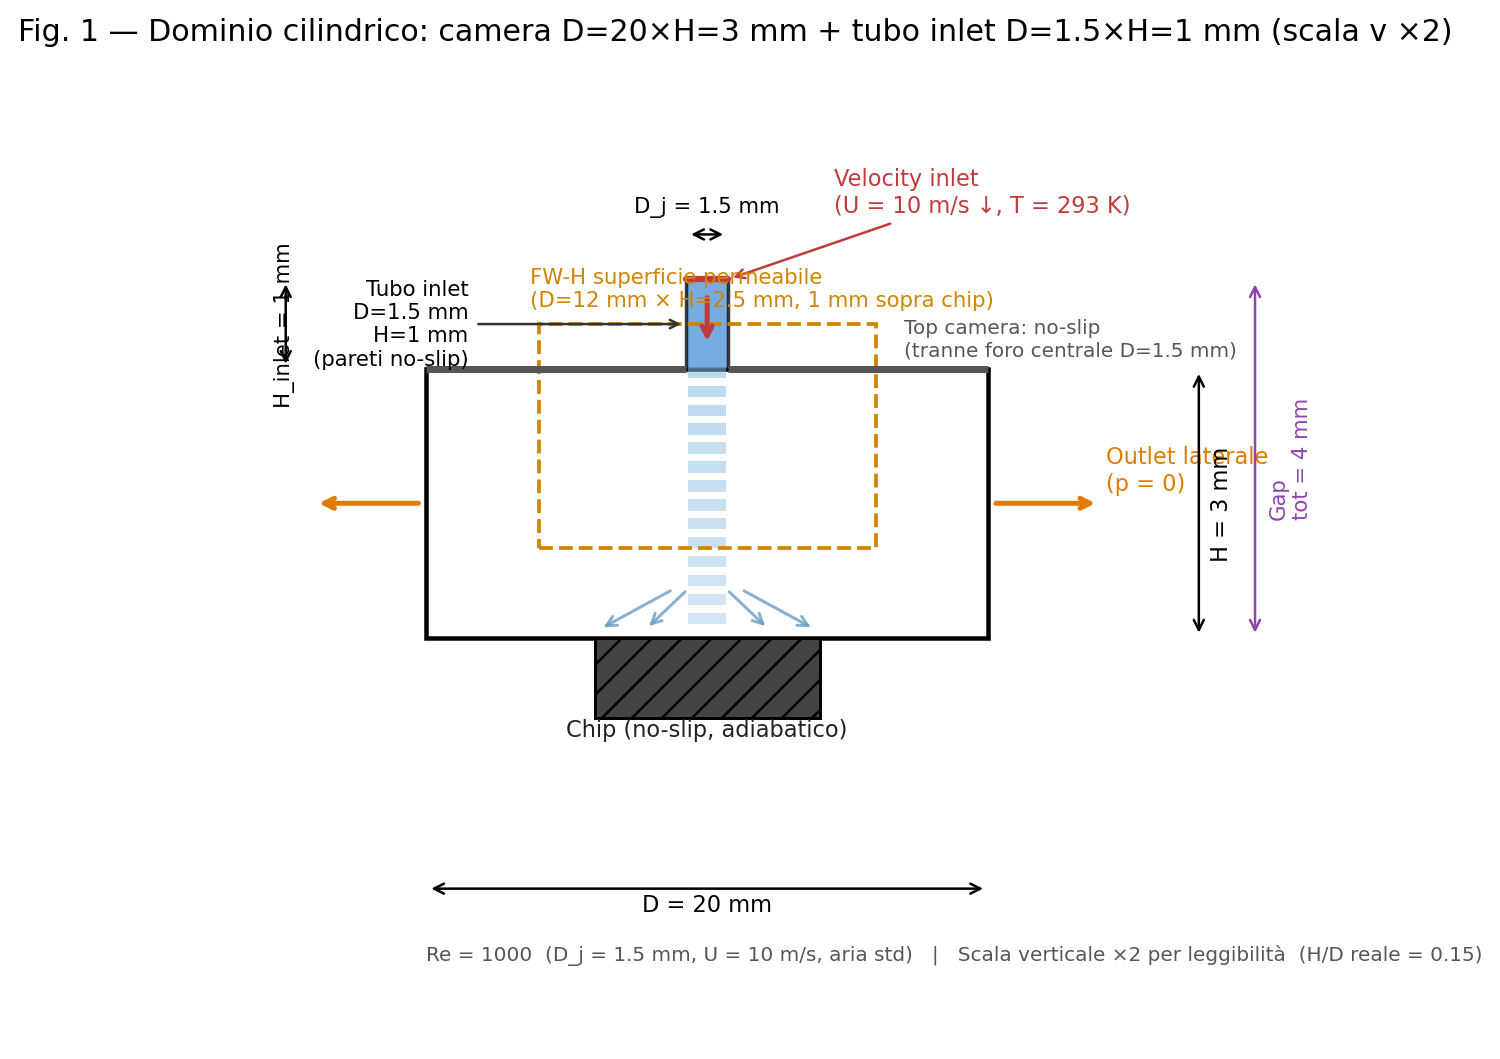
\includegraphics[width=0.80\textwidth]{fig_domain}
    \captionof{figure}{Schema della geometria di simulazione: camera cilindrica (D=20\,mm, H=3\,mm), tubo di inlet (D=1.5\,mm), chip sul fondo e superficie laterale come outlet a pressione nulla.}
  \end{center}

  \vfill
  {\color{huaweiblue}\rule{\linewidth}{1.5pt}}
  \vspace{0.3cm}
  {\small\color{midblue}
    Documento riservato --- uso interno Huawei Research Finland / Università di Genova
  }
\end{titlepage}

% -------- SOMMARIO ESECUTIVO --------
\newpage
\section*{Sommario Esecutivo}
\addcontentsline{toc}{section}{Sommario Esecutivo}

Il presente documento descrive il setup completo per la simulazione CFD aeroacustica di un getto d'aria impingente su chip di smartphone, commissionata da Huawei Research Center Finland al Prof.\ Bottaro dell'Università di Genova. Il problema fisico riguarda il raffreddamento forzato di chip top-gamma tramite jet ad impatto diretto: la configurazione garantisce un'efficienza termica elevata, ma genera un rumore udibile nell'intervallo 1--20\,kHz che risulta fastidioso per l'utente finale.

\textbf{Geometria.} Il dominio è compatto: una camera cilindrica di diametro 20\,mm e altezza 3\,mm, con un tubo di inlet coassiale di diametro 1.5\,mm. Il chip occupa il fondo della camera (superficie circolare D=20\,mm). La velocità di iniezione è $U=10$\,m/s, corrispondente a $\Rey = 1000$ e $\Ma = 0.029$; il regime è incompressibile ed è pertanto applicabile l'analogia acustica di Ffowcs-Williams \& Hawkings.

\textbf{Approccio numerico.} La pipeline di validazione si articola in sei fasi: RANS SST (convergenza, Grid Convergence Index), URANS (analisi spettrale di Strouhal), DDES (verifica cascata energetica $-5/3$), WMLES, WRLES e post-processing FW-H. Il solver target è SU2 v8 in modalità incompressibile (\ttcfg{INC\_NAVIER\_STOKES}) con modello sottogriglia WALE per la fase LES.

\textbf{Mesh.} La mesh non strutturata ibrida è generata con Ennova (mesher del committente), secondo una progressione di 8 livelli da 150\,k celle (debug) a 60--100\,M celle (DNS aspirazionale). Il caso principale è il livello L5 (WRLES, 12\,M celle, $\Delta x_{\min}=20\mum$).

\textbf{Hardware e costi.} Il laptop del committente (AMD Ryzen 9 AI 370 HX, 24 thread) è adatto per la fase RANS fino a L3 (3\,M celle, 50--70\,h). Le simulazioni LES richiedono HPC: il percorso minimo fino alla WRLES costa circa €1.590 su CINECA (accademico) o \$2.740 su AWS Spot.

\textbf{Roadmap.} Il programma di lavoro si sviluppa in 4 mesi: fase RANS su laptop nel primo mese, URANS/DDES nel secondo, WMLES+WRLES su HPC nel terzo e quarto. Il documento contiene template completi di configurazione SU2 (RANS e LES), criteri di qualità mesh, stime di costo dettagliate e decisioni progettuali aperte.

\vspace{0.4cm}
\hrule
\vspace{0.4cm}
{\small
\textbf{Nota sulla proprietà intellettuale.} Il codice SU2 è rilasciato con licenza LGPL v2.1 (open source). I risultati della simulazione e il know-how sviluppato nel corso della commessa appartengono a Huawei Research Center Finland secondo i termini contrattuali vigenti. Il presente documento ha scopo tecnico-illustrativo e non costituisce offerta commerciale.
}

% -------- TABLE OF CONTENTS --------
\newpage
\tableofcontents
\newpage

% ============================================================
\section{Contesto e Obiettivi}
\label{sec:contesto}
% ============================================================

\subsection{Il problema del raffreddamento nei chip top-gamma}

I chip di ultima generazione per smartphone (SoC da 3\,nm e oltre) dissipano potenze nell'ordine di 10--15\,W in picchi sostenuti durante gaming o elaborazione AI on-device. La riduzione del nodo tecnologico aumenta la densità di integrazione ma riduce proporzionalmente la superficie di scambio termico disponibile, rendendo la convezione naturale insufficiente a mantenere la giunzione sotto la temperatura massima di 90--100\,°C.

La soluzione esplorata da Huawei Research Center Finland è la \textbf{convezione forzata tramite jet impingente}: un ugello di piccolo diametro ($\Djet = 1.5$\,mm) dirige un flusso d'aria ad alta velocità direttamente sulla superficie del chip. L'efficienza termica di questo schema è eccellente --- il coefficiente di scambio locale nella zona di impatto può superare $h = 500$\,W/(m$^2$K), ordini di grandezza sopra la convezione libera --- ma la velocità elevata nel getto e l'interazione con le pareti generate \textbf{rumore dipolare e quadrupolare} nell'intervallo udibile.

\subsection{Il tradeoff acustico-termico}

Gli esperimenti condotti presso il laboratorio Huawei hanno evidenziato due configurazioni limite:

\begin{description}
  \item[Configurazione A (jet libero, senza mesh):] getto diretto sull'inlet, nessun elemento ostruttivo. Coefficiente termico massimo, ma rumore percepito dall'utente nell'intervallo 2--15\,kHz. Il livello di pressione sonora (SPL) misurato a 10\,cm supera i 45--50\,dBSPL in condizioni di picco \cite{Viswanathan2004}.

  \item[Configurazione B (jet con mesh cubica):] una griglia di celle cubiche di lato $\approx 0.5$\,mm è posizionata davanti all'inlet. La mesh degrada e distribuisce la coerenza vortici nel getto, riducendo il rumore di circa 10--15\,dB. Il costo è una riduzione del $\approx 20$--30\% del coefficiente di scambio termico medio.
\end{description}

Il problema di ottimizzazione è trovare geometrie intermedie (forma dell'ugello, distanza chip--inlet, possibile geometria del deflettore) che massimizzino $h_{\mathrm{medio}}$ sotto vincolo di SPL massimo ammissibile. Questa ottimizzazione richiede un modello CFD aeroacustico validato.

\subsection{Scope della commessa}

La commessa iniziale ha uno scope ben definito e conservativo:

\begin{enumerate}
  \item \textbf{Riproduzione al CFD della configurazione A} (jet libero, senza mesh cubica), replicando le condizioni geometriche e di flusso del setup sperimentale Huawei.
  \item \textbf{Validazione quantitativa} del campo di flusso (profili di velocità media, fluttuazioni RMS, numero di Strouhal del getto) contro le misure PIV/hot-wire disponibili.
  \item \textbf{Predizione del campo acustico far-field} tramite analogia FW-H applicata a superfici di controllo nella zona di impatto \cite{Shur2005}.
\end{enumerate}

Le commesse future (condizionali al successo della validazione) includono: parametric sweep della geometria dell'ugello, studio della configurazione B con mesh cubica, ottimizzazione forma-acustica del deflettore. Questi step richiedono un tool CFD affidabile e validato, da costruire nella presente fase.

\subsection{Il solver SU2}

SU2 \cite{Economon2016} è un codice open-source per la simulazione multifisica sviluppato originariamente presso Stanford University e ora mantenuto da una comunità internazionale. Il solver è già stato utilizzato dal gruppo di ricerca per simulazioni RANS sub/supersoniche, garantendo continuità di competenza. Per il presente progetto sono rilevanti:

\begin{itemize}
  \item Il solutore incompressibile (\ttcfg{INC\_NAVIER\_STOKES}) basato su splitting pressione-velocità di tipo SIMPLE/SIMPLEC.
  \item Il modello di turbolenza SST di Menter per la fase RANS.
  \item I modelli ibridi RANS-LES: SA-DDES (\cite{Spalart2006}) e WALE per la fase LES (\cite{Nicoud1999}).
  \item L'analogia acustica di Ffowcs-Williams \& Hawkings integrata nel codice (\ttcfg{ACOUSTIC\_ANALOGY= FWH}) \cite{Zhou2018}.
\end{itemize}

% ============================================================
\section{Inquadramento Fisico}
\label{sec:fisica}
% ============================================================

\subsection{Parametri adimensionali di regime}

Il fluido di lavoro è aria standard a 20\,°C con le proprietà riportate in Tabella~\ref{tab:fluid}.

\begin{table}[H]
  \centering
  \caption{Proprietà fisiche dell'aria a 20\,°C, 1\,atm.}
  \label{tab:fluid}
  \rowcolors{2}{lightblue!40}{white}
  \begin{tabular}{llcl}
    \toprule
    \rowcolor{tablehead}
    \textbf{Grandezza} & \textbf{Simbolo} & \textbf{Valore} & \textbf{Unità} \\
    \midrule
    Densità           & $\rho$          & 1.225          & kg/m$^3$ \\
    Viscosità dinamica & $\mu$          & $1.8375\times10^{-5}$ & Pa$\cdot$s \\
    Viscosità cinematica & $\nu$        & $1.5\times10^{-5}$ & m$^2$/s \\
    Velocità del suono & $c$            & 343            & m/s \\
    Temperatura inlet  & $T_0$          & 293.15         & K \\
    \bottomrule
  \end{tabular}
\end{table}

I parametri adimensionali chiave sono:
\begin{align}
  \Rey &= \frac{\rho\, U\, \Djet}{\mu}
       = \frac{1.225 \times 10 \times 1.5\times10^{-3}}{1.8375\times10^{-5}}
       = 1000 \label{eq:re} \\
  \Ma  &= \frac{U}{c}
       = \frac{10}{343}
       = 0.029 \label{eq:ma}
\end{align}

Il numero di Reynolds $\Rey = 1000$ colloca il flusso nel regime di transizione/turbolenza debole: il getto si sviluppa con turbolenza confinata prevalentemente nello strato di taglio anulare, senza la piena cascata inerziale dei jet ad alto Re. Il numero di Mach $\Ma \approx 0.03$ è abbondantemente infrasonic: l'ipotesi di incompressibilità introdotta nelle equazioni di governo è valida, con correzioni comprimibili dell'ordine di $\Ma^2 \approx 0.001$ (0.1\%).

\subsection{Regime del getto confinato e numero di Strouhal}

Il rapporto tra distanza chip--inlet e diametro del getto è:
\begin{equation}
  H/\Djet = \frac{3\,\text{mm}}{1.5\,\text{mm}} = 2
\end{equation}
(oppure $H/\Djet = 2.67$ considerando anche la lunghezza del tubo di inlet). Questo colloca il caso nel \textbf{regime confined impinging jet}: il getto impatta sul chip prima di aver completato lo sviluppo turbolento in aria libera.

Il numero di Strouhal atteso per le oscillazioni del getto (vortex shedding dalla bocca dell'ugello) è:
\begin{equation}
  \Str = \frac{f\,\Djet}{U} \approx 0.1\text{--}0.4
  \quad\Rightarrow\quad
  f \approx 670\text{--}2670\,\text{Hz}
\end{equation}
Questa banda è integralmente nell'udibile (20--20\,000\,Hz) e corrisponde alle frequenze di disturbo percepite dall'utente.

\subsection{Meccanismi di generazione del rumore}

In un getto impingente incompressibile i principali meccanismi acustici sono:

\begin{description}
  \item[Sorgenti dipolari di parete:] la fluttuazione di pressione sul chip e sul top della camera genera emissione dipolare (forze fluttuanti su superfici rigide). Questo è il contributo dominante a basso Mach \cite{FfowcsHawkings1969}.
  \item[Sorgenti quadrupolari nel fluido:] le fluttuazioni di Reynolds stress nel getto generano rumore quadrupolare, proporzionale a $\Ma^5$. A $\Ma = 0.03$ è trascurabile rispetto al contributo dipolare.
  \item[Feedback aeroelastico (possibile):] l'impingement può generare un loop di feedback tra il getto e la camera risonante, con toni discreti sovrapposti allo spettro a banda larga.
\end{description}

\subsection{Formulazione incompressibile con acustica FW-H}

L'approccio numerico adottato disaccoppia il campo aerodinamico near-field dall'emissione acustica far-field:

\begin{enumerate}
  \item \textbf{Campo near-field:} soluzione delle equazioni di Navier--Stokes incompressibili con modello SGS (fase LES) su dominio compatto.
  \item \textbf{Far-field acustico:} integrazione dell'analogia FW-H sull'equazione di Lighthill estesa, utilizzando le fluttuazioni di pressione e velocità estratte da una superficie di controllo $S_{\mathrm{FW-H}}$ posizionata attorno alla zona di impatto.
\end{enumerate}

L'equazione di Ffowcs-Williams \& Hawkings per superfici impermeabili in moto relativo è \cite{FfowcsHawkings1969}:
\begin{equation}
  \square^2 p'(\mathbf{x},t) =
  \frac{\partial}{\partial t}\left[\rho_0 v_n\, \delta(f)\right]
  - \frac{\partial}{\partial x_i}\left[l_i\, \delta(f)\right]
  + \frac{\partial^2}{\partial x_i\partial x_j}\left[T_{ij}\, H(f)\right]
\end{equation}
dove $v_n$ è la velocità normale alla superficie, $l_i = (p - p_0)\hat{n}_i + \rho u_i(u_j-v_j)\hat{n}_j$ sono le forze di superficie, $T_{ij}$ il tensore di Lighthill e $\square^2 = \nabla^2 - c^{-2}\partial^2/\partial t^2$ l'operatore d'onda. A Mach basso il termine quadrupolare $T_{ij}$ è trascurabile e SU2 integra solo i primi due contributi.

% ============================================================
\section{Geometria e Condizioni al Contorno}
\label{sec:geometria}
% ============================================================

\subsection{Descrizione del dominio}

Il dominio computazionale è composto da due regioni cilindriche coassiali (Figura~\ref{fig:domain_body}):

\begin{itemize}
  \item \textbf{Camera principale:} cilindro di diametro $\Dcam = 20$\,mm e altezza $\Hcam = 3$\,mm. Il chip occupa la superficie circolare inferiore ($z=0$).
  \item \textbf{Tubo di inlet:} cilindro di diametro $\Djet = 1.5$\,mm e altezza $H_{\mathrm{tube}} = 1$\,mm, montato coassialmente sul centro del top della camera ($z = 3$\,mm), con il top del tubo a $z = 4$\,mm.
\end{itemize}

\begin{figure}[H]
  \centering
  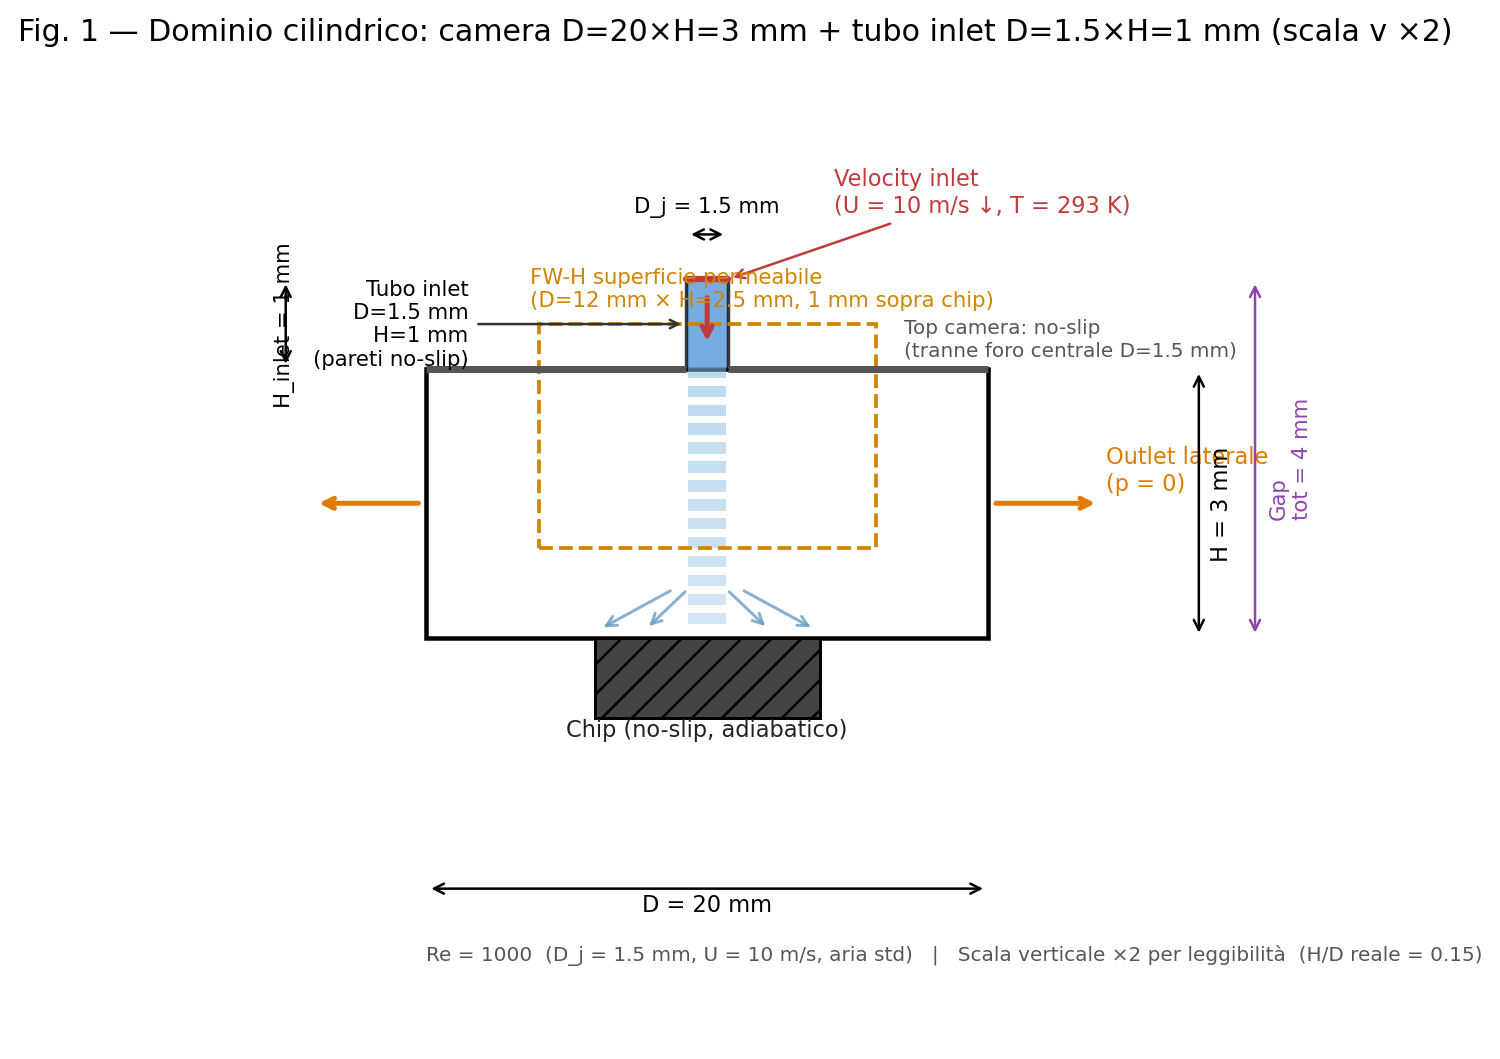
\includegraphics[width=0.80\textwidth]{fig_domain}
  \caption{Geometria del dominio: camera cilindrica (grigio), tubo inlet (blu), chip (arancio), frecce rosse indicano la direzione del flusso. La superficie di controllo FW-H (verde tratteggiato) è indicata schematicamente.}
  \label{fig:domain_body}
\end{figure}

\subsection{Dimensioni caratteristiche}

\begin{table}[H]
  \centering
  \caption{Dimensioni geometriche del dominio e rapporti adimensionali.}
  \label{tab:geometria}
  \rowcolors{2}{lightblue!40}{white}
  \begin{tabular}{llcc}
    \toprule
    \rowcolor{tablehead}
    \textbf{Elemento} & \textbf{Dimensione} & \textbf{Valore} & \textbf{Unità} \\
    \midrule
    Diametro camera      & $\Dcam$               & 20              & mm \\
    Altezza camera       & $\Hcam$               & 3               & mm \\
    Diametro tubo inlet  & $\Djet$               & 1.5             & mm \\
    Altezza tubo inlet   & $H_{\mathrm{tube}}$   & 1               & mm \\
    Distanza top-tubo -- chip & $H_{\mathrm{tot}}$ & 4            & mm \\
    Gap effettivo (fondo tubo -- chip) & $H_{\mathrm{gap}}$ & 3 & mm \\
    Rapporto $H_{\mathrm{gap}}/\Djet$ & ---        & 2               & --- \\
    Rapporto $H_{\mathrm{tot}}/\Djet$ & ---        & 2.67            & --- \\
    Rapporto $\Dcam/\Djet$            & ---        & 13.3            & --- \\
    \bottomrule
  \end{tabular}
\end{table}

\subsection{Condizioni al contorno}

Le condizioni al contorno sono specificate per ogni marker della mesh (Tabella~\ref{tab:bc}) e riportate anche nel template di configurazione SU2 alla Sezione~\ref{sec:config}.

\begin{table}[H]
  \centering
  \caption{Condizioni al contorno e marker SU2 corrispondenti.}
  \label{tab:bc}
  \rowcolors{2}{lightblue!40}{white}
  \begin{tabularx}{\textwidth}{lllX}
    \toprule
    \rowcolor{tablehead}
    \textbf{Superficie} & \textbf{Tipo} & \textbf{Marker SU2} & \textbf{Dettagli} \\
    \midrule
    Top del tubo inlet ($\phi$=1.5\,mm) & Velocity inlet & \ttcfg{jet\_inlet} & $U=10$\,m/s in $-z$, $T=293.15$\,K, profilo uniforme \\
    Parete laterale tubo & No-slip adiabatica & \ttcfg{inlet\_tube\_wall} & \ttcfg{MARKER\_HEATFLUX= 0.0} \\
    Top camera (anello, foro D=1.5\,mm) & No-slip adiabatica & \ttcfg{top\_plate} & \ttcfg{MARKER\_HEATFLUX= 0.0} \\
    Parete laterale camera ($\phi$=20\,mm, H=3\,mm) & Pressure outlet & \ttcfg{lateral\_outlet} & $p_{\mathrm{gauge}} = 0$\,Pa \\
    Chip (fondo camera, $\phi$=20\,mm) & No-slip adiabatica & \ttcfg{chip\_wall} & \ttcfg{MARKER\_HEATFLUX= 0.0} (fase futura: heat flux imposto) \\
    \bottomrule
  \end{tabularx}
\end{table}

\textbf{Nota sulla condizione di inlet.} Il profilo di velocità uniforme (plug flow) è una semplificazione conservativa. In realtà il tubo di inlet ha lunghezza 1\,mm e diametro 1.5\,mm ($L/D = 0.67$), insufficiente a sviluppare un profilo di Poiseuille. Un profilo turbolento sviluppato richiederebbe $L/D \gtrsim 10$--20. La scelta di un profilo plug è coerente con un inlet pressurizzato a monte, come tipicamente realizzato nel setup sperimentale con ugello raccordato.

\textbf{Condizione termica sul chip.} La simulazione di validazione adotta una parete adiabatica (\ttcfg{MARKER\_HEATFLUX= 0.0}). In un secondo momento, la commessa prevede l'imposizione di un flusso termico $q'' = 5\text{--}15$\,W/cm$^2$ per lo studio del raffreddamento accoppiato. SU2 supporta questa condizione tramite \ttcfg{MARKER\_HEATFLUX} con valore negativo in convezione (flusso dal solido al fluido) o tramite temperatura di parete imposta (\ttcfg{MARKER\_ISOTHERMAL}).

% ============================================================
\section{Scale di Turbolenza}
\label{sec:scale}
% ============================================================

\subsection{Gerarchia delle scale: dalla cascata energetica a Kolmogorov}

La turbolenza del getto confinato genera strutture vorticose su scale molto diverse, dalla scala integrale (dell'ordine del diametro del getto) fino alla microscala di Kolmogorov (dissipazione viscosa). La comprensione di questa gerarchia è essenziale per la progettazione della mesh e del passo temporale.

\begin{figure}[H]
  \centering
  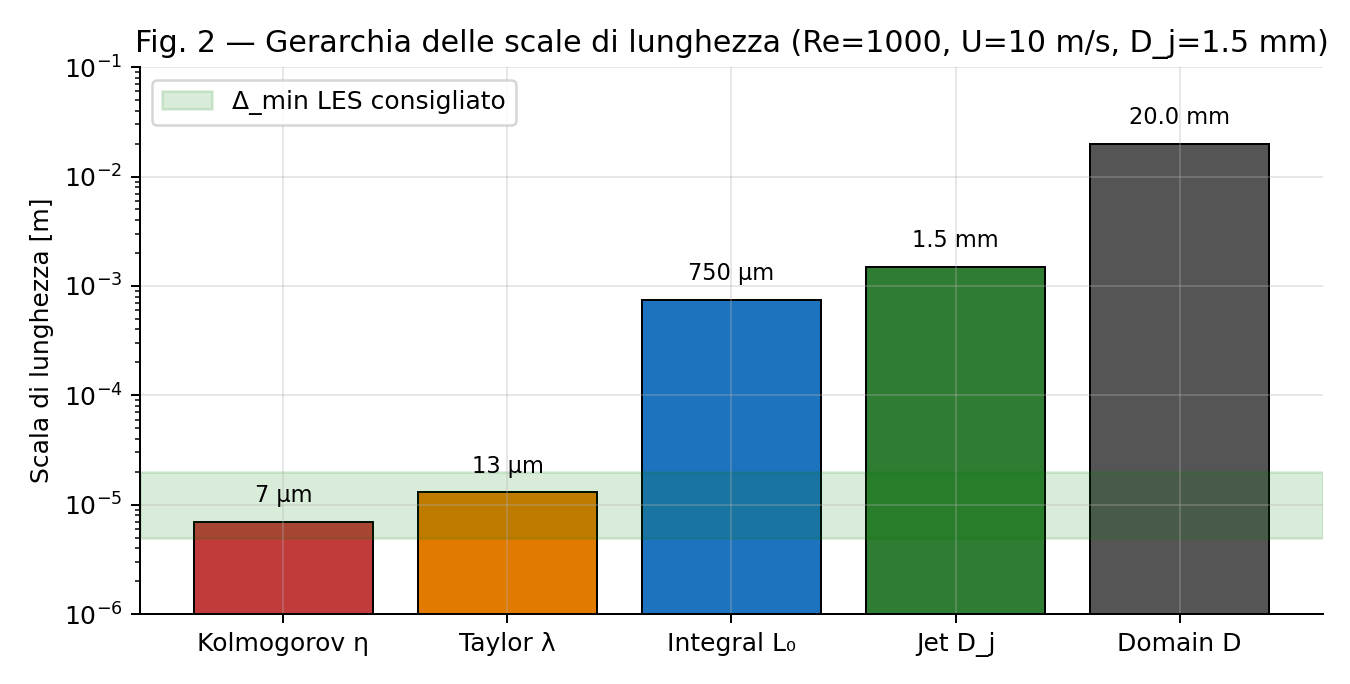
\includegraphics[width=0.88\textwidth]{fig_scales}
  \caption{Gerarchia delle scale turbolente nel getto impingente: scala integrale $L_0$, microscala di Taylor $\lambda$, scala di Kolmogorov $\eta$. In rosso i limiti di risoluzione dei vari livelli di mesh.}
  \label{fig:scales}
\end{figure}

\subsection{Calcolo delle scale caratteristiche}

Le stime seguenti sono riferite alla zona di shear layer del getto, dove la turbolenza è più intensa.

\textbf{Scala integrale.} La scala di lunghezza integrale è stimata come una frazione del diametro del getto:
\begin{equation}
  L_0 \approx \frac{\Djet}{2} = 0.75\,\text{mm}
\end{equation}

\textbf{Tasso di dissipazione turbolenta.} Nella zona di strato di taglio, il tasso di dissipazione è stimato tramite:
\begin{equation}
  \varepsilon \approx \frac{U^3}{L_0}
  = \frac{(10)^3}{7.5\times10^{-4}}
  = 1.33\times10^{6}\,\text{m}^2/\text{s}^3
\end{equation}

\textbf{Scala di Kolmogorov.} La microscala di Kolmogorov $\eta$ rappresenta la dimensione delle strutture dissipative:
\begin{equation}
  \eta = \left(\frac{\nu^3}{\varepsilon}\right)^{1/4}
       = \left(\frac{(1.5\times10^{-5})^3}{1.33\times10^{6}}\right)^{1/4}
       \approx 7\mum
\end{equation}

\textbf{Microscala di Taylor.} La microscala di Taylor $\lambda$ è definita tramite:
\begin{equation}
  \lambda = \sqrt{\frac{15\nu\,u'^2}{\varepsilon}}
\end{equation}
con $u' \approx 1$\,m/s (fluttuazione di velocità RMS nella zona di shear, $\approx 10\%$ di $U$):
\begin{equation}
  \lambda = \sqrt{\frac{15 \times 1.5\times10^{-5} \times 1}{1.33\times10^{6}}}
          \approx 13\mum
\end{equation}

\textbf{Numero di Reynolds turbolento.} Il numero di Reynolds basato sulla scala di Taylor è:
\begin{equation}
  Re_\lambda = \frac{u'\,\lambda}{\nu}
             = \frac{1 \times 1.3\times10^{-5}}{1.5\times10^{-5}}
             \approx 0.87
\end{equation}
Questo valore molto basso ($Re_\lambda \ll 10$) indica che la turbolenza è \textbf{debolmente sviluppata}: le scale di Taylor e di Kolmogorov sono dello stesso ordine di grandezza, e il range inerziale (che normalmente si estende tra $L_0$ e $\eta$ per $Re_\lambda \gg 1$) è praticamente assente. Questo ha importanti implicazioni: le simulazioni RANS e LES sono meno accuratamente separabili, e il modello SGS gioca un ruolo ridotto rispetto ad un getto ad alto Re.

\textbf{Scale temporali.} Le scale temporali caratteristiche sono:
\begin{align}
  \tau_\eta   &= \left(\frac{\nu}{\varepsilon}\right)^{1/2}
               = \left(\frac{1.5\times10^{-5}}{1.33\times10^6}\right)^{1/2}
               \approx 3.4\mus \\
  \tau_{\mathrm{jet}} &= \frac{\Djet}{U}
               = \frac{1.5\times10^{-3}}{10}
               = 150\mus \\
  \tFT         &\approx \frac{H_{\mathrm{cam}}}{U_{\mathrm{bulk,radiale}}}
               \approx 4\,\text{ms}
\end{align}
dove $\tFT$ è il \emph{flow-through time} stimato considerando che la velocità bulk nella camera è circa 1\,m/s (il getto deve uscire radialmente dalla camera, riducendo la velocità media di un fattore $\sim\Djet^2/\Dcam^2 \approx 1/180$).

\begin{table}[H]
  \centering
  \caption{Riepilogo delle scale turbolente nel getto impingente.}
  \label{tab:scales}
  \rowcolors{2}{lightblue!40}{white}
  \begin{tabular}{llcc}
    \toprule
    \rowcolor{tablehead}
    \textbf{Scala} & \textbf{Simbolo} & \textbf{Valore} & \textbf{Unità} \\
    \midrule
    Scala integrale     & $L_0$        & 0.75      & mm \\
    Microscala di Taylor & $\lambda$    & 13        & $\mu$m \\
    Scala di Kolmogorov  & $\eta$       & 7         & $\mu$m \\
    Tempo di Kolmogorov  & $\tau_\eta$  & 3.4       & $\mu$s \\
    Tempo convettivo jet & $\tau_{\mathrm{jet}}$ & 150 & $\mu$s \\
    Flow-through time   & $\tFT$       & 4         & ms \\
    Durata simulazione  & $10\,\tFT$   & 40        & ms \\
    $Re_\lambda$        & ---          & $\approx 0.87$ & --- \\
    \bottomrule
  \end{tabular}
\end{table}

% ============================================================
\section{Passo Temporale}
\label{sec:timestep}
% ============================================================

\subsection{Analisi dei vincoli}

La scelta del passo temporale $\Delta t$ deve soddisfare contemporaneamente i seguenti vincoli (Figura~\ref{fig:timestep}):

\begin{figure}[H]
  \centering
  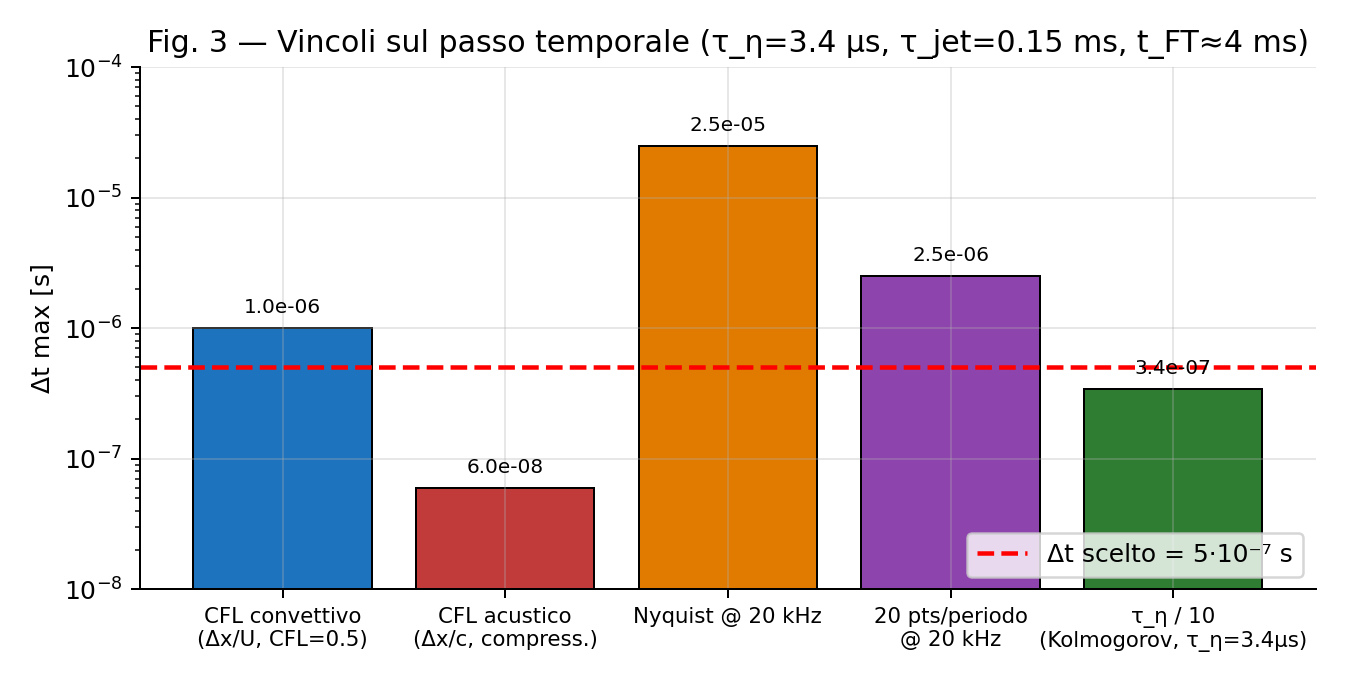
\includegraphics[width=0.88\textwidth]{fig_timestep}
  \caption{Vincoli sul passo temporale: CFL convettivo (blu), criterio di Nyquist a 20\,kHz (verde), 20 punti per periodo a 20\,kHz (arancio), scala temporale di Kolmogorov $\tau_\eta/10$ (rosso). Il passo scelto è indicato dalla linea tratteggiata.}
  \label{fig:timestep}
\end{figure}

\textbf{Vincolo 1 — CFL convettivo.} Per la mesh fine (livello L5, $\Delta x_{\min} = 30\mum$ nella zona bulk), con $U = 10$\,m/s e CFL = 0.5:
\begin{equation}
  \Delta t \leq \frac{\mathrm{CFL}\,\Delta x}{U}
  = \frac{0.5 \times 30\times10^{-6}}{10}
  = 1.5\mus
\end{equation}

\textbf{Vincolo 2 — Nyquist a 20\,kHz.} La frequenza massima di interesse acustico è $f_{\max} = 20$\,kHz:
\begin{equation}
  \Delta t \leq \frac{1}{2f_{\max}}
  = \frac{1}{2 \times 20000}
  = 25\mus
\end{equation}

\textbf{Vincolo 3 — 20 punti per periodo a 20\,kHz.} Per una rappresentazione accurata dello spettro fino a 20\,kHz con almeno 20 campioni per periodo:
\begin{equation}
  \Delta t \leq \frac{1}{20\,f_{\max}}
  = 2.5\mus
\end{equation}

\textbf{Vincolo 4 — Scala temporale di Kolmogorov.} Per la LES wall-resolved, il passo temporale deve risolvere le strutture dissipative:
\begin{equation}
  \Delta t \leq \frac{\tau_\eta}{10}
  = \frac{3.4\mus}{10}
  = 0.34\mus
  \quad \leftarrow \text{vincolo dominante}
\end{equation}

\subsection{Passo temporale scelto}

Il passo temporale adottato per la simulazione WRLES principale (livello L5) è:
\begin{equation}
  \boxed{\Delta t_{\mathrm{LES}} = 5\times10^{-7}\,\text{s} = 0.5\mus}
\end{equation}

Questo valore è leggermente più conservativo di $\tau_\eta/10$ (0.34\,$\mu$s), ma più conveniente computazionalmente (numero intero di step per i flow-through time). Il numero di CFL effettivo sulla mesh L5 ($\Delta x_{\min} = 20\mum$ nelle celle bulk):
\begin{equation}
  \mathrm{CFL}_{\mathrm{eff}} = \frac{U\,\Delta t}{\Delta x}
  = \frac{10 \times 5\times10^{-7}}{20\times10^{-6}}
  = 0.25
\end{equation}
valore conservativo, compatibile con la stabilità dello schema temporale DUAL\_TIME\_STEPPING-2ND\_ORDER di SU2.

\begin{table}[H]
  \centering
  \caption{Riepilogo dei vincoli sul passo temporale e confronto con $\Delta t$ scelto.}
  \label{tab:timestep}
  \rowcolors{2}{lightblue!40}{white}
  \begin{tabular}{lcc}
    \toprule
    \rowcolor{tablehead}
    \textbf{Vincolo} & \textbf{Limite superiore $\Delta t$} & \textbf{Soddisfatto?} \\
    \midrule
    CFL convettivo ($\Delta x=30\mum$, CFL=0.5) & $1.5\mus$  & \checkmark \\
    Nyquist @ 20\,kHz                            & $25\mus$   & \checkmark \\
    20 punti/periodo @ 20\,kHz                   & $2.5\mus$  & \checkmark \\
    $\tau_\eta/10$ (Kolmogorov)                  & $0.34\mus$ & \checkmark \\
    \midrule
    \textbf{$\Delta t$ scelto (WRLES L5)}        & $\mathbf{0.5\,\mu s}$ & --- \\
    \bottomrule
  \end{tabular}
\end{table}

Per le simulazioni a minor fedeltà (RANS, URANS, DDES) i passi temporali sono più grandi, come dettagliato nella Tabella~\ref{tab:simparams} alla Sezione~\ref{sec:simparams}.

% ============================================================
\section{Mesh Non Strutturata con Ennova}
\label{sec:mesh}
% ============================================================

\subsection{Mesher Ennova}

Il mesher target del committente è \textbf{Ennova} (SimScale/Numeca group), un generatore di mesh non strutturata ibrida prism+tet ottimizzato per domini fluidodinamici con strati limite curvilinei. Le principali caratteristiche rilevanti per questo caso sono:

\begin{itemize}
  \item \textbf{Prism layers anisotropi:} crescita geometrica degli strati prism vicino a parete, con controllo di $y^+$ tramite impostazione del primo layer e del growth rate.
  \item \textbf{Raffinamento locale volumetrico:} box e sferette di raffinamento attorno alla zona di shear layer del getto.
  \item \textbf{Export SU2:} Ennova esporta direttamente in formato \texttt{.su2} (Sezione~\ref{sec:workflow}).
  \item \textbf{Compatibilità con GCI:} il parametro di raffinamento $r$ è controllabile globalmente tra i livelli di mesh, garantendo la coerenza con il metodo di Celik \cite{Celik2008} per il Grid Convergence Index.
\end{itemize}

\subsection{Struttura della mesh ibrida}

La mesh è composta da due regioni strutturalmente distinte:

\begin{description}
  \item[Zona di parete (prism layers):] strati prismatici ortogonali alla parete per la risoluzione degli strati limite. Il primo layer ha altezza $\Delta y_1$ calcolata per ottenere il $y^+$ target. Il growth rate è tipicamente 1.15--1.25 tra layer consecutivi.
  \item[Zona bulk (tetraedri + esaedri):] tetraedri irregolari nel volume lontano da parete, con raffinamento progressivo nella zona del getto (shear layer anulare) e nella zona di impatto (stagnation point sul chip).
\end{description}

La stima del primo layer per il $y^+$ target è ottenuta dall'equazione di van Driest (valida per $y^+ < 5$):
\begin{equation}
  \Delta y_1 = \frac{y^+\,\nu}{u_\tau}
  \qquad\text{con}\quad
  u_\tau = U\sqrt{\frac{C_f}{2}}
  \approx U\sqrt{\frac{0.079}{2\,\Rey^{0.25}}}
\end{equation}
Per $\Rey = 1000$ e $U = 10$\,m/s: $u_\tau \approx 0.54$\,m/s, $\Delta y_1(y^+=1) \approx 28\mum$, $\Delta y_1(y^+=0.5) \approx 14\mum$.

\subsection{Progressione dei livelli di mesh}

La Tabella~\ref{tab:mesh} descrive gli 8 livelli di raffinamento progressivo, dal debug al DNS aspirazionale. Il rapporto di raffinamento tra livelli consecutivi è $r = 1.5$--$2$, compatibile con il criterio di Celik per il GCI.

\begin{figure}[H]
  \centering
  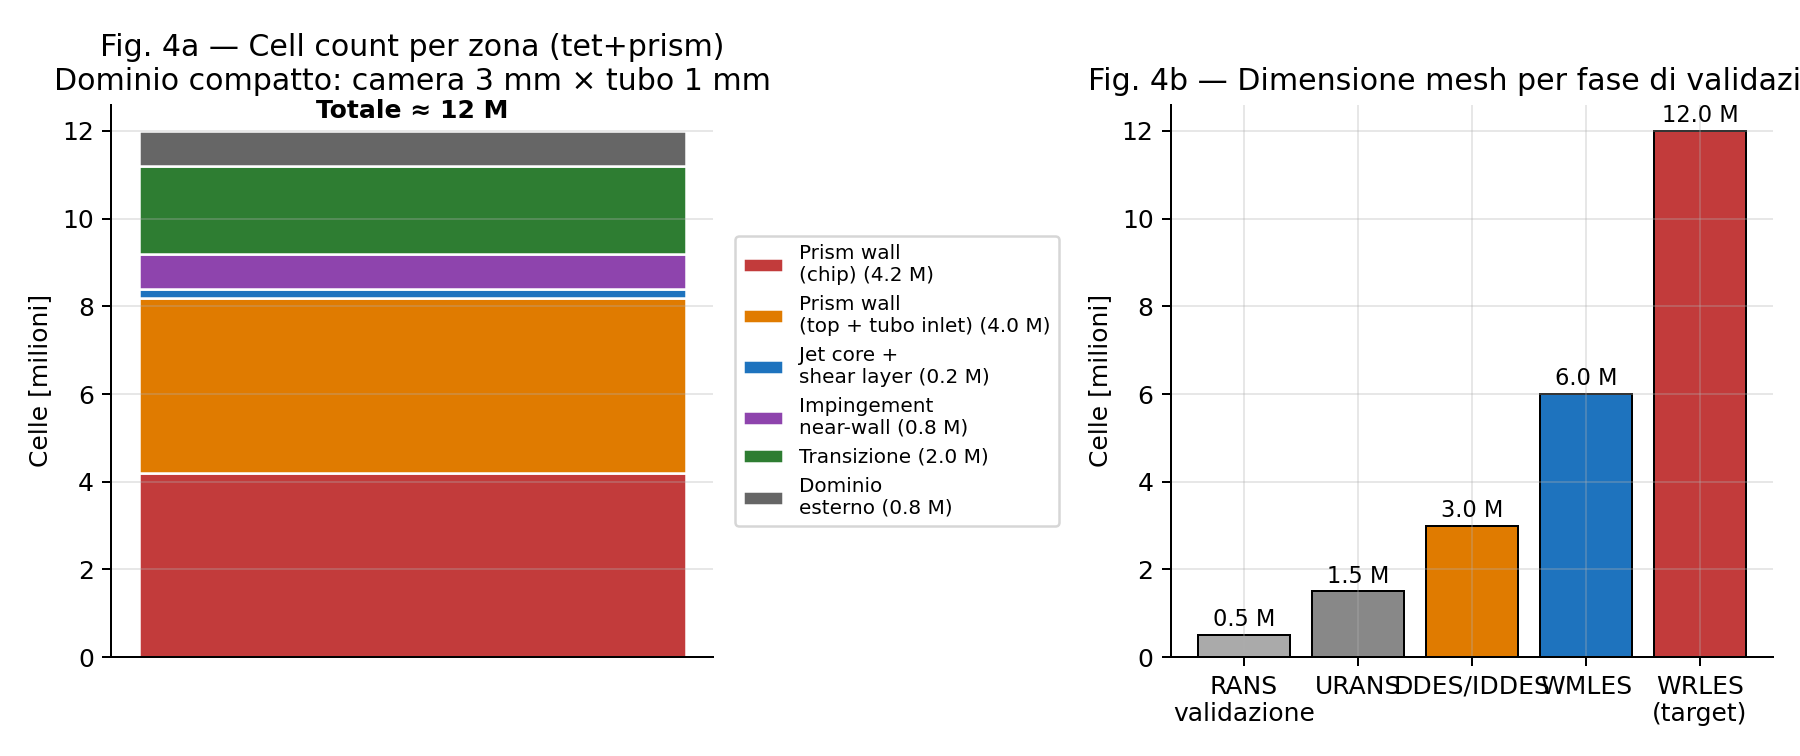
\includegraphics[width=\textwidth]{fig_cells}
  \caption{Breakdown del numero di celle per livello di mesh (sinistra) e confronto relativo alla capacità hardware (destra). Il gap tra laptop e HPC per la fase LES è evidente.}
  \label{fig:cells}
\end{figure}

\begin{longtable}{p{1.8cm}rp{1.2cm}p{1.2cm}p{1.2cm}p{1.3cm}p{2.0cm}p{2.0cm}}
  \caption{Progressione dei livelli di mesh da debug a DNS. $N_c$: numero di celle; $\Delta x_w$: dimensione minima cella a parete; $\Delta x_b$: dimensione bulk; $N_{PL}$: strati prism.}
  \label{tab:mesh} \\
  \toprule
  \rowcolor{tablehead}
  \textbf{Livello} & $\mathbf{N_c}$ & $\mathbf{\Delta x_w}$ & $\mathbf{\Delta x_b}$ & $\mathbf{N_{PL}}$ & $\mathbf{y^+}$ max & \textbf{Uso} & \textbf{HW target} \\
  \midrule
  \endfirsthead
  \toprule
  \rowcolor{tablehead}
  \textbf{Livello} & $\mathbf{N_c}$ & $\mathbf{\Delta x_w}$ & $\mathbf{\Delta x_b}$ & $\mathbf{N_{PL}}$ & $\mathbf{y^+}$ max & \textbf{Uso} & \textbf{HW target} \\
  \midrule
  \endhead
  \bottomrule
  \endfoot
  L0 Debug & 150\,k & 200\,$\mu$m & 500\,$\mu$m & 5 & $\sim$5 & Test BC, geom. & Laptop (30\,min) \\
  L1 RANS coarse & 500\,k & 80\,$\mu$m & 300\,$\mu$m & 8 & $\sim$2 & RANS SST & Laptop (8--10\,h) \\
  L2 RANS medium & 1.5\,M & 50\,$\mu$m & 200\,$\mu$m & 10 & $\sim$1.5 & RANS GCI, URANS & Laptop (24--30\,h) \\
  L3 RANS fine & 3\,M & 30\,$\mu$m & 150\,$\mu$m & 10 & $\sim$1 & GCI fine, DDES & Laptop/HPC \\
  L4 WMLES base & 6\,M & 25\,$\mu$m & 100\,$\mu$m & 8 & $\sim$30 (wm) & WMLES WALE & HPC 128--256\,c \\
  L5 WRLES target & 12\,M & 20\,$\mu$m & 80\,$\mu$m & 12 & $<$0.5 & WRLES WALE & HPC 256--512\,c \\
  L6 WRLES verif. & 20\,M & 15\,$\mu$m & 60\,$\mu$m & 14 & $<$0.3 & Check ind. mesh & HPC 512--1024\,c \\
  L7 DNS aspiraz. & 60--100\,M & 7\,$\mu$m & 21\,$\mu$m & 16 & $<$0.2 & DNS full & HPC 2048+\,c \\
\end{longtable}

\subsection{Critici di qualità mesh}

\textbf{Aspect ratio.} Le celle prism vicino a parete hanno aspect ratio elevato (tipicamente 20--100): questo è normale e desiderabile per la risoluzione dello strato limite, ma richiede un numerics robusto (schema WEIGHTED\_LEAST\_SQUARES per i gradienti in SU2).

\textbf{Non-orthogonality.} La transizione da prism a tet può generare celle con angoli non ortogonali $>60°$. Ennova offre un tool di smoothing che riduce il $P_{90}$ della non-ortogonalità a valori $<45°$, accettabili per SU2.

\textbf{Skewness.} Celle con skewness $>0.8$ (Fluent convention) o equiangle skew $>70°$ devono essere eliminate. La zona di transizione prism-tet richiede attenzione.

\textbf{Volume ratio.} Il rapporto di volume tra celle adiacenti non deve superare 10--15 per evitare oscillazioni numeriche nelle zone di forte raffinamento.

\subsection{Nota sul regime WMLES vs WRLES}

I livelli L4 (WMLES) e L5 (WRLES) differiscono non solo nel numero di celle ma nella filosofia di modellazione di parete:

\begin{itemize}
  \item \textbf{WMLES ($y^+ \approx 30$):} le celle di parete non risolvono lo strato viscoso; viene usato un modello di parete algebraico per fornire lo stress a parete alla LES. Il modello è accurato in flussi non separati e in equilibrio, ma introduce errore in zona di impatto (forte decelerazione).
  \item \textbf{WRLES ($y^+ < 0.5$):} la mesh risolve esplicitamente il sottostrato viscoso ($y^+ < 5$) e la zona buffer ($5 < y^+ < 30$). Non è necessario alcun modello di parete. L'accuratezza è massima, a costo di un fattore $\sim 2$ in numero di celle.
\end{itemize}

Per il caso di impingement confinato, la zona di stagnation point è critica: il flusso impatta ortogonalmente la parete e la turbolenza non è in equilibrio locale \cite{Hadziabdic2008}. La DNS di riferimento di Dairay et al.\ \cite{Dairay2015} mostra che gli errori WMLES in questa zona possono superare il 15\% sul Nusselt number locale. La WRLES è pertanto il caso principale della commessa.

% ============================================================
\section{Simulazioni Instazionarie: \texorpdfstring{$\Delta t$}{Dt} e Steps}
\label{sec:simparams}
% ============================================================

\subsection{Parametri per ciascuna simulazione}

La Tabella~\ref{tab:simparams} riassume i parametri temporali per ciascun livello di fedeltà.

\begin{table}[H]
  \centering
  \caption{Parametri delle simulazioni instazionarie: passo temporale, durata fisica, numero di step, iterazioni inner e livello di mesh.}
  \label{tab:simparams}
  \rowcolors{2}{lightblue!40}{white}
  \begin{tabularx}{\textwidth}{lXXXXXX}
    \toprule
    \rowcolor{tablehead}
    \textbf{Sim} & $\Delta t$ & \textbf{Dur.} & $N_{\mathrm{step}}$ & $N_{\mathrm{inner}}$ & $N_c$ & \textbf{Note} \\
    \midrule
    URANS SST   & $10\mus$ & 60\,ms & 6\,000  & 30 & 1.5\,M (L2) & FFT pressione, Strouhal \\
    DDES SA     & $5\mus$  & 40\,ms & 8\,000  & 25 & 3\,M (L3)   & Verifica spettro $-5/3$ \\
    WMLES WALE  & $1\mus$  & 40\,ms & 40\,000 & 20 & 6\,M (L4)   & Primo check Pope M \\
    WRLES WALE  & $0.5\mus$& 50\,ms & 100\,000 & 20 & 12\,M (L5) & Caso principale \\
    \bottomrule
  \end{tabularx}
\end{table}

\textbf{Strategia di inizializzazione.} Ogni simulazione a fedeltà più alta è inizializzata dalla soluzione stazionaria/instazionaria del livello precedente:

\begin{itemize}
  \item URANS SST: inizializzato dalla soluzione RANS converged (L2).
  \item DDES SA: inizializzato dalla URANS dopo 3\,$\tFT$ di flushout.
  \item WMLES: inizializzato dalla DDES interpolata sulla mesh L4.
  \item WRLES: inizializzato dalla WMLES interpolata sulla mesh L5, con 10\,ms di flushout (\emph{preflush} = $2.5\,\tFT$) scartati prima di avviare la raccolta delle statistiche.
\end{itemize}

\subsection{Dettaglio URANS SST (L2)}

\begin{description}
  \item[Obiettivo:] primo segnale instazionario, identificazione del numero di Strouhal, verifica della periodicità/quasi-periodicità del getto.
  \item[$\Delta t = 10\mus$:] $\approx 1/5$ del periodo di Strouhal atteso ($f \approx 670$\,Hz $\rightarrow T \approx 1.5$\,ms). La risoluzione temporale è modesta ma sufficiente per cogliere il contenuto spettrale fino a $f \approx 2.5$\,kHz.
  \item[Raccolta dati:] pressione sul chip e sull'outlet campionate ogni step; elaborazione FFT dopo il transiente di assestamento (primi 2\,$\tFT$ = 8\,ms scartati, ultimi 52\,ms = 13\,$\tFT$ per la statistica).
  \item[Crit. di convergenza inner:] riduzione residui di almeno 3 ordini entro 30 iterazioni; se non raggiunto entro 30, il passo è accettato con warning.
\end{description}

\subsection{Dettaglio DDES SA (L3)}

La DDES (Delayed Detached Eddy Simulation) di Spalart et al. \cite{Spalart2006} utilizza il modello SA (Spalart-Allmaras) come base RANS nelle zone di parete (dove la mesh non risolve la turbolenza) e attiva il modo LES nelle zone lontane da parete (shear layer libero del getto). La separazione dipende da una funzione di shielding $f_d$ che inibisce la commutazione RANS→LES nelle celle attaccate alla parete.

\begin{itemize}
  \item Parametro chiave: \ttcfg{KIND\_TURB\_MODEL= SA} con \ttcfg{DDES= YES}.
  \item Il modello SA è calibrato per flussi a bassa separazione; in impingement la stagnation point anomaly può essere rilevante. Confronto con SST-DDES consigliato come sensitivity check.
  \item L'obiettivo principale del livello DDES è verificare la presenza della cascata energetica $-5/3$ nello spettro di velocità nella zona di shear layer ($x/\Djet \approx 0.5$--$1.5$).
\end{itemize}

\subsection{Dettaglio WMLES e WRLES WALE}

Il modello SGS WALE (Wall-Adapting Local Eddy-viscosity) \cite{Nicoud1999} è scelto per le sue proprietà:

\begin{enumerate}
  \item La viscosità SGS si azzera correttamente vicino a parete ($\mu_{\mathrm{sgs}} \propto y^3$), senza la sovra-attivazione del modello di Smagorinsky standard.
  \item Non richiede la procedura di van Driest damping.
  \item È computazionalmente economico (solo operazioni sui gradienti locali).
\end{enumerate}

La viscosità eddy SGS del modello WALE è:
\begin{equation}
  \mu_{\mathrm{sgs}} = \rho\left(C_w\,\Delta\right)^2
  \frac{\left(S_{ij}^d\,S_{ij}^d\right)^{3/2}}
  {\left(\bar{S}_{ij}\bar{S}_{ij}\right)^{5/2}+\left(S_{ij}^d\,S_{ij}^d\right)^{5/4}}
\end{equation}
dove $S_{ij}^d$ è la parte simmetrica del quadrato del tensore gradiente di velocità, $\bar{S}_{ij}$ è il tensore di deformazione media, $\Delta = V_c^{1/3}$ è la scala della cella e $C_w = 0.325$ (valore di default in SU2).

% ============================================================
\section{Pipeline di Validazione Multi-Fedeltà}
\label{sec:pipeline}
% ============================================================

\subsection{Struttura della pipeline}

La validazione è organizzata in 6 fasi sequenziali, ciascuna con input, criteri di accettazione e output definiti (Figura~\ref{fig:pipeline}). Una fase non si avvia se la precedente non ha soddisfatto i propri criteri.

\begin{figure}[H]
  \centering
  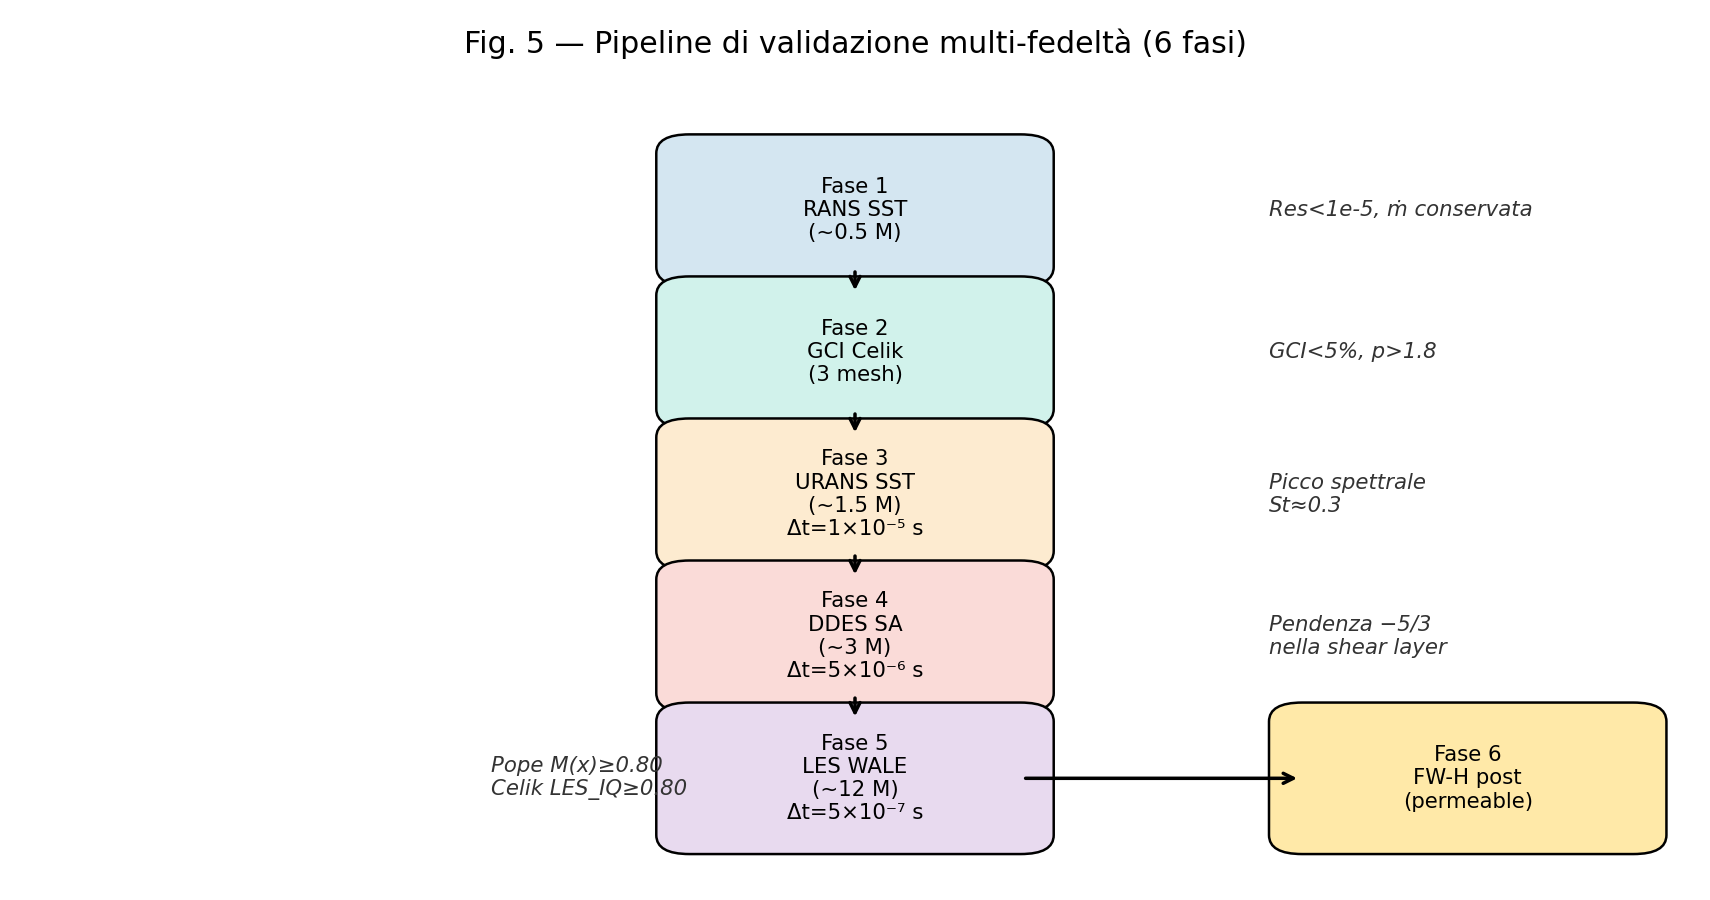
\includegraphics[width=\textwidth]{fig_pipeline}
  \caption{Pipeline di validazione a 6 fasi: da RANS grossolano a post-processing FW-H. Frecce verdi indicano le dipendenze; box rossi le verifiche di qualità.}
  \label{fig:pipeline}
\end{figure}

\subsection{Fase 1 — RANS SST: Convergenza e GCI}

\textbf{Obiettivo:} campo di flusso stazionario su tre livelli di mesh (L1, L2, L3) per la verifica della convergenza di griglia tramite Grid Convergence Index (GCI) secondo Celik et al.\ \cite{Celik2008}.

\textbf{Quantità di interesse (QoI):} velocità assiale media al centro del jet a $z/H=0.5$ ($\bar{u}_{z,c}$), coefficiente di pressione sul chip ($C_p$), separazione di flusso alla periferia della camera.

\textbf{Metodo GCI.} Per tre soluzioni $\phi_1$ (fine), $\phi_2$ (medium), $\phi_3$ (coarse) con rapporti di raffinamento $r_{21}$ e $r_{32}$:
\begin{align}
  p &= \frac{\ln\left[(\phi_3-\phi_2)/(\phi_2-\phi_1)\right]}{\ln r} \\
  \phi_{\mathrm{ext}} &= \phi_1 + \frac{\phi_1 - \phi_2}{r^p - 1} \\
  \mathrm{GCI}_{\mathrm{fine}} &= \frac{1.25\,|(\phi_2-\phi_1)/\phi_1|}{r^p-1}
\end{align}

\textbf{Criterio di accettazione:} $\mathrm{GCI}_{\mathrm{fine}} < 3\%$ sulla QoI principale.

\subsection{Fase 2 — URANS SST: Analisi Spettrale}

\textbf{Obiettivo:} identificare il numero di Strouhal del getto e verificare la risposta in frequenza del dominio.

\textbf{Metodo:} FFT della pressione superficiale sul chip (punto centrale e punto a $r = \Djet/4$ dal centro). Lunghezza FFT $\geq 2^{13}$ punti per risoluzione spettrale $\Delta f \leq 2$\,Hz.

\textbf{Criteri:} picco spettrale a $\Str \in [0.1, 0.4]$; armonica dominante identificata; assenza di aliasing (verifica Nyquist).

\subsection{Fase 3 — DDES SA: Cascata Energetica}

\textbf{Obiettivo:} verificare la presenza del range inerziale ($-5/3$) nello spettro di energia turbolenta nella zona di shear layer.

\textbf{Metodo:} spettro di potenza della velocità assiale a $r = \Djet/4$, $z = H/2$; confronto con slope teorica $E(f) \propto f^{-5/3}$.

\textbf{Criteri:} slope -5/3 riconoscibile su $\geq 1$ decade di frequenza; transizione verso il range dissipativo visibile a $f \sim 1/\tau_\eta$.

\textbf{Nota:} con $Re_\lambda \approx 0.87$ il range inerziale sarà breve (meno di un'ottava). Il criterio è pertanto qualitativo: la DDES deve mostrare una tendenza alla slope -5/3, non necessariamente un range esteso.

\subsection{Fase 4 — WMLES WALE: Pope M-index}

\textbf{Obiettivo:} prima simulazione LES su mesh L4; verifica della risoluzione tramite Pope M-index \cite{Pope2000}.

Il Pope M-index è definito come la frazione di energia turbolenta risolta dalla LES:
\begin{equation}
  M = \frac{k_{\mathrm{risolto}}}{k_{\mathrm{risolto}} + k_{\mathrm{sgs}}}
  \geq 0.80 \quad \text{(criterio di Pope)}
\end{equation}
dove $k_{\mathrm{sgs}} = \mu_{\mathrm{sgs}}\,\bar{S}_{ij}\,\bar{S}_{ij}/\rho$ e $k_{\mathrm{risolto}} = \frac{1}{2}\langle u_i'u_i'\rangle$.

\textbf{Criterio:} $M > 0.80$ in almeno il 90\% del volume computazionale. Zone di $M < 0.80$ localizzate all'outlet sono tollerate.

\subsection{Fase 5 — WRLES WALE: Statistiche Convergenti}

\textbf{Obiettivo:} simulazione principale, raccolta statistiche per confronto con misure sperimentali Huawei.

\textbf{Quantità estratte:}
\begin{itemize}
  \item Profili radiali di $\bar{u}_z(r)$ a diverse quote $z$ (confronto con PIV).
  \item Fluttuazioni RMS $u'_z(r)$, $u'_r(r)$.
  \item Nusselt number locale $\mathrm{Nu}(r)$ sul chip (caso futuro con heat flux).
  \item Spettro di pressione superficiale sul chip e sull'outlet.
\end{itemize}

\textbf{Convergenza statistica:} statistiche raccolte su $\geq 8\,\tFT = 32$\,ms di soluzione. La convergenza è verificata confrontando statistiche su primo e secondo semi-intervallo (criterio di stationarity).

\subsection{Fase 6 — Post-processing FW-H}

\textbf{Obiettivo:} calcolo del campo acustico far-field tramite analogia FW-H.

\textbf{Superficie FW-H:} superficie chiusa posizionata a $r = 1.5\,\Dcam/2 = 15$\,mm dal chip, racchiudente la zona di impatto. L'integrazione avviene in SU2 tramite \ttcfg{ACOUSTIC\_ANALOGY= FWH}.

\textbf{Punti osservatori:} definiti nel file \texttt{fwh\_observers.dat}, tipicamente su arco emisferico a $r = 100\,\Dcam = 2$\,m (simulazione far-field acustico).

\textbf{Output:} SPL$(f)$ in dBSPL alla frequenza di riferimento $p_{\mathrm{ref}} = 20\,\mu$Pa, per confronto diretto con le misure sperimentali Huawei (microfono a 10\,cm dal chip).

% ============================================================
\section{Hardware: Laptop vs Supercomputer}
\label{sec:hardware}
% ============================================================

\subsection{Laptop del committente: AMD Ryzen 9 AI 370 HX}

\begin{figure}[H]
  \centering
  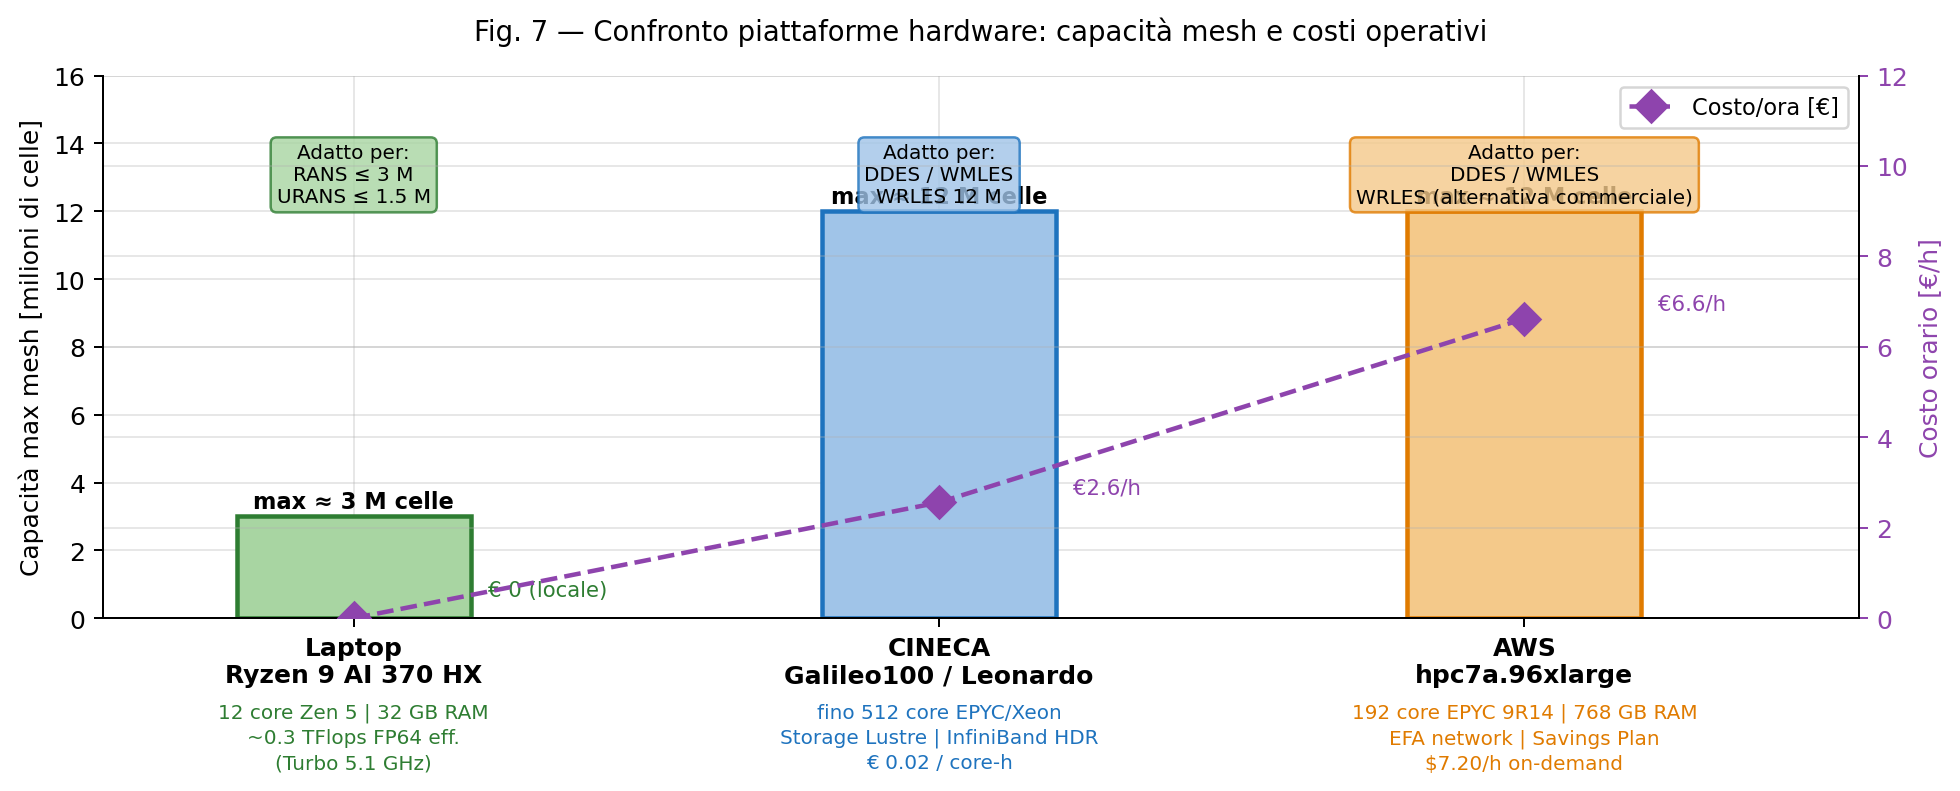
\includegraphics[width=\textwidth]{fig_hardware}
  \caption{Confronto delle capacità hardware: laptop AMD Ryzen 9 AI 370 HX (sinistra), cluster CINECA Leonardo (centro), istanza AWS hpc7a (destra). Barre verdi: simulazioni accessibili; barre arancio: borderline; barre rosse: non praticabili.}
  \label{fig:hardware}
\end{figure}

Il laptop del committente è basato su un SoC AMD Ryzen 9 AI 370 HX con architettura Zen\,5/Zen\,5c (nodo TSMC N4P, 2024). Le specifiche rilevanti per SU2 sono:

\begin{table}[H]
  \centering
  \caption{Specifiche hardware del laptop del committente.}
  \label{tab:laptop}
  \rowcolors{2}{lightblue!40}{white}
  \begin{tabular}{ll}
    \toprule
    \rowcolor{tablehead}
    \textbf{Componente} & \textbf{Specifica} \\
    \midrule
    CPU & AMD Ryzen 9 AI 370 HX (Zen\,5 + Zen\,5c hybrid) \\
    Core fisici & 12 (4 Zen\,5 ``performance'' + 8 Zen\,5c ``efficiency'') \\
    Thread logici (SMT) & 24 \\
    Clock boost Zen\,5 & fino a 5.1\,GHz \\
    Clock base Zen\,5c & 3.3\,GHz \\
    Performance FP64 (SU2, sostenuto) & $\approx 0.25$--0.35\,TFLOPS \\
    RAM & 32\,GB DDR5-7500 dual-channel \\
    Larghezza banda memoria & $\approx 120$\,GB/s \\
    NPU XDNA 2 & 50\,TOPS (non usabile da SU2) \\
    GPU integrata & AMD Radeon 890M RDNA\,3.5 (non usabile da SU2) \\
    TDP configurabile & 28--55\,W \\
    \bottomrule
  \end{tabular}
\end{table}

\textbf{Limitazioni pratiche per SU2.}

\begin{itemize}
  \item \textbf{Memoria:} SU2 incompressibile alloca circa 1.0--1.5\,kB/cella per il campo di soluzione, più i buffer MPI, gli strati halo e i gradienti. Con 32\,GB RAM, il limite pratico è circa 12--15\,M celle. Le simulazioni LES L5 (12\,M) sono teoricamente in limite di memoria.
  \item \textbf{Efficienza parallela:} con 10--12 core attivi e partizionamento METIS, l'efficienza parallela è 70--80\%. Il core ottimo per SU2 su Ryzen\,9 è circa 8--10 core fisici (i Zen\,5c hanno minore performance per double-precision FP64).
  \item \textbf{Wall-time:} la stima di performance è 8--12\,$\mu$s/cella/inner-iter su core moderno. Per L3 RANS (3\,M celle, 5\,000 iter, 1 inner/iter): $3\times10^6 \times 5000 \times 10\mus / 10 \approx 150$\,h.
  \item \textbf{Throttling termico:} il TDP massimo di 55\,W è difficilmente sostenibile per giorni in laptop non raffreddati adeguatamente. In pratica, il TDP stabile è 35--40\,W, riducendo le performance del 15--20\%.
\end{itemize}

\textbf{Capacità realistica:}
\begin{itemize}
  \item RANS L0--L2: \checkmark\ OK (ore--giorni)
  \item RANS L3 (3\,M celle): \checkmark\ possibile ma lento (50--70\,h)
  \item URANS L2 (1.5\,M, $\Delta t=10\mus$, 6\,000 step): circa 3--4 giorni
  \item DDES L3 (3\,M, $\Delta t=5\mus$, 8\,000 step): $\geq 7$ giorni (borderline)
  \item WMLES L4 in poi: \textbf{non praticabile} (tempo $>30$ giorni, memoria borderline)
\end{itemize}

\subsection{HPC accademico: CINECA Leonardo}

CINECA è il consorzio universitario italiano che gestisce i più grandi supercomputer nazionali. L'accesso accademico è disponibile tramite convenzione con l'Università di Genova.

\textbf{Leonardo DCGP (Data-Centric General Purpose):}
\begin{itemize}
  \item Processori: AMD EPYC 7763 (Milan, Zen\,3), 64 core per socket, 128 core per nodo
  \item RAM per nodo: 512\,GB DDR4-3200 (8 canali)
  \item Interconnessione: InfiniBand HDR200 (200\,Gb/s) a bassa latenza
  \item Storage parallelo: IBM Spectrum Scale (GPFS), $>100$\,GB/s aggregate
  \item Pricing accademico (ISCRA grant): $\approx$€0.020/core-h
  \item Pricing commerciale (ICE): $\approx$€0.045/core-h
  \item Wall-time massimo per job: 24\,h (con possibilità di checkpoint e resubmit)
  \item Coda tipica: 24--48\,h in condizioni normali di carico
\end{itemize}

\textbf{Galileo100 (alternativa):}
\begin{itemize}
  \item Processori: Intel Xeon Platinum 8260 (Cascade Lake), 24 core per socket
  \item Nodi a 48 core, 384\,GB RAM
  \item Pricing accademico: $\approx$€0.015/core-h
  \item Adatto per job fino a 256 core; per 512 core consigliato Leonardo
\end{itemize}

\textbf{Accesso:} la richiesta di allocazione ISCRA-C (sino a 100\,kcore-h) è relativamente rapida (2--4 settimane). L'Università di Genova ha una convenzione attiva con CINECA. Il Prof.\ Bottaro può co-sponsorizzare la richiesta.

\subsection{HPC cloud: AWS EC2 HPC}

Per chi necessita di flessibilità immediata (senza attesa coda accademica), le istanze HPC di AWS offrono accesso in minuti.

\begin{table}[H]
  \centering
  \caption{Confronto istanze AWS EC2 HPC rilevanti.}
  \label{tab:aws}
  \rowcolors{2}{lightblue!40}{white}
  \begin{tabularx}{\textwidth}{lXXXX}
    \toprule
    \rowcolor{tablehead}
    \textbf{Istanza} & \textbf{vCPU} & \textbf{RAM} & \textbf{Rete} & \textbf{Prezzo} \\
    \midrule
    hpc7a.96xlarge & 192 EPYC 9R14 (Genoa) & 768\,GB & 300\,Gbps EFA & \$7.20/h (OD), \$2.30/h (Spot) \\
    hpc6a.48xlarge & 96 EPYC 7R13 (Milan) & 384\,GB & 100\,Gbps EFA & \$2.88/h (OD), \$1.00/h (Spot) \\
    c7i.24xlarge & 96 Intel Sapphire Rapids & 192\,GB & 50\,Gbps & \$4.28/h (OD) \\
    \bottomrule
  \end{tabularx}
\end{table}

\textbf{Configurazione consigliata per WRLES L5 (512 vCPU):} 3$\times$ hpc7a.96xlarge in cluster con EFA (Elastic Fabric Adapter). Il networking EFA riduce la latenza MPI a valori paragonabili all'InfiniBand. Costo spot: $3\times\$2.30/\text{h} = \$6.90/\text{h}$.

\textbf{Storage:} le simulazioni LES generano output voluminosi ($\approx 5$--10\,GB ogni 1\,000 step × 200\,step di output = 10--20\,GB per simulazione). Usare FSx Lustre ($0.15/\text{GB-mese}$) per I/O parallelo; scaricare i risultati su S3 ($0.023/\text{GB-mese}$) prima di terminare l'istanza. I costi di egress (uscita da AWS) sono $0.09/\text{GB}$: da considerare nel budget.

\subsection{Altre opzioni HPC}

\begin{description}
  \item[Rescale:] piattaforma HPC-as-a-service con SU2 pre-installato e interfaccia web per il lancio di job. Costo $0.05$--$0.15/\text{core-h}$; adatto per utenti senza esperienza di HPC Linux. Conveniente per job brevi ma costoso per job lunghi rispetto ad AWS.
  \item[Google Cloud HPC (H3/C3):] istanze Intel Sapphire Rapids con interconnessione Titanium (RDMA), costo $\approx\$0.04$--$0.05/\text{vCPU-h}$. MPI over RDMA richiede configurazione specifica.
  \item[Azure HBv4:] 176 core AMD EPYC Genoa per nodo, InfiniBand NDR, \$3.60/h commitment. Buona opzione se il committente ha già un contratto Azure enterprise.
\end{description}

% ============================================================
\section{Stima Tempi e Costi}
\label{sec:costi}
% ============================================================

\subsection{Modello di performance}

La stima dei tempi di calcolo si basa sul modello:
\begin{equation}
  t_{\mathrm{wall}} = \frac{N_c \times N_{\mathrm{step}} \times N_{\mathrm{inner}} \times t_{\mathrm{cell}}}
                          {N_{\mathrm{core}} \times \eta_p}
\end{equation}
dove $t_{\mathrm{cell}} \approx 8\,\mu\text{s/cella/iter}$ (SU2 INC\_NS su core Zen\,3/Zen\,4 moderno) e $\eta_p \approx 0.75$ è l'efficienza parallela stimata.

I core-h totali per una simulazione sono:
\begin{equation}
  \text{Core-h} = N_{\mathrm{core}} \times t_{\mathrm{wall}}
\end{equation}

\begin{figure}[H]
  \centering
  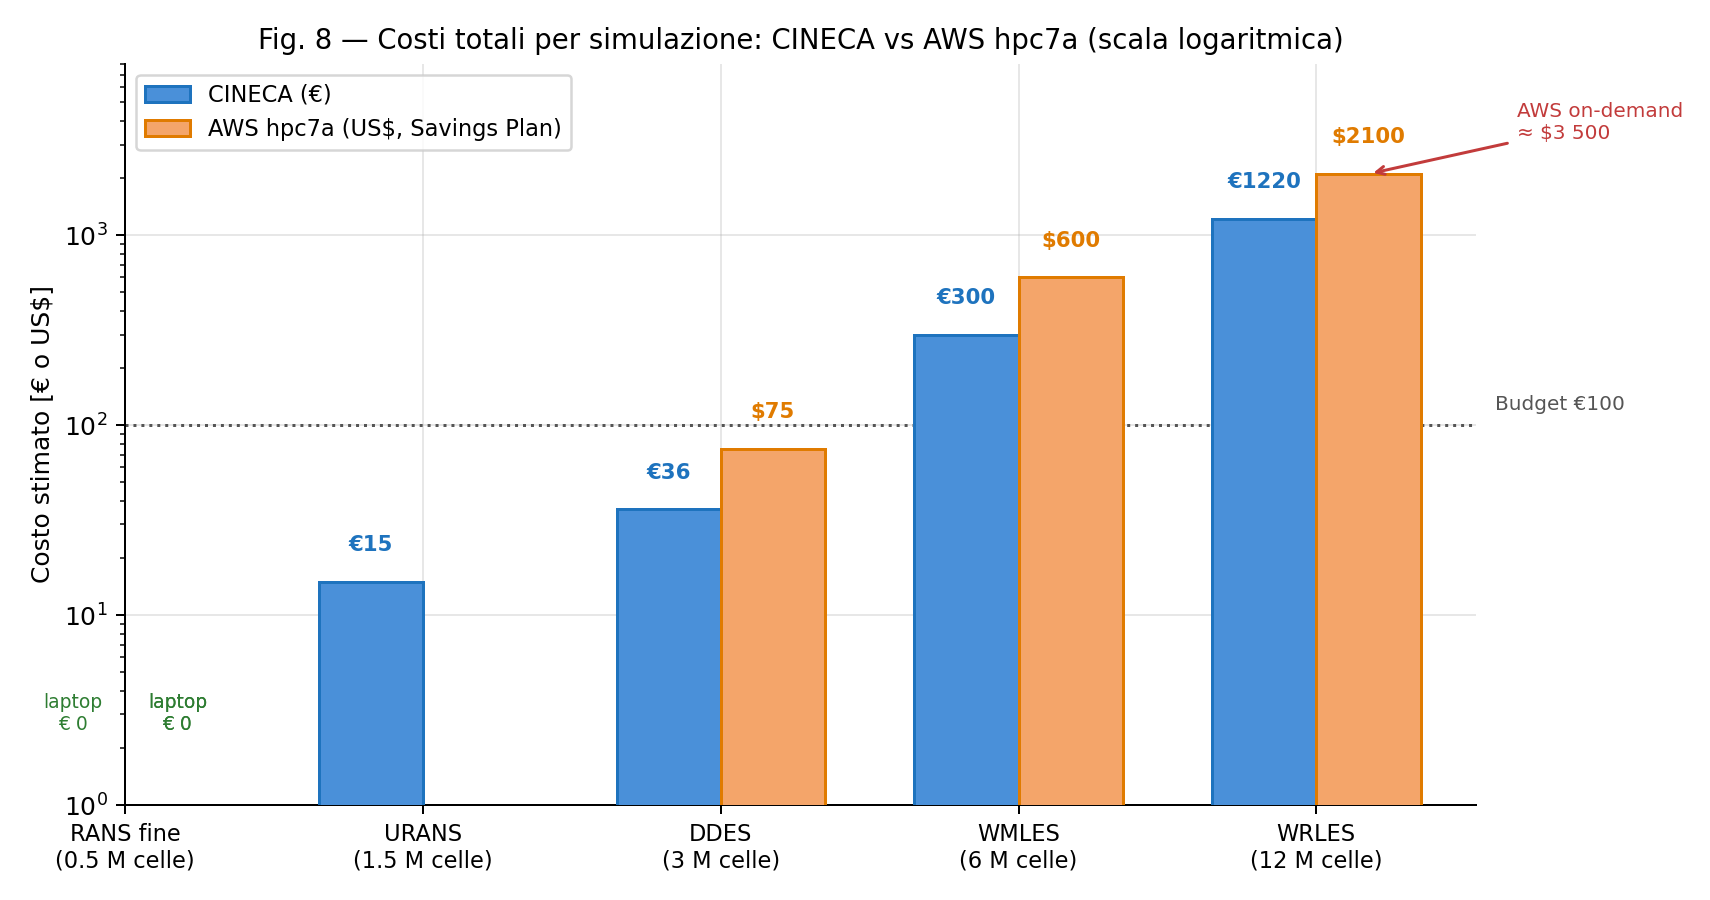
\includegraphics[width=\textwidth]{fig_costs}
  \caption{Confronto dei costi stimati per ciascun livello di simulazione su CINECA (accademico), AWS Spot e AWS On-Demand. I costi LES (L4--L6) dominano il budget complessivo.}
  \label{fig:costs}
\end{figure}

\subsection{Tabella dei costi per simulazione}

\begin{longtable}{p{1.5cm}p{0.9cm}p{2.2cm}p{2.0cm}p{1.3cm}p{1.5cm}p{1.8cm}p{1.8cm}}
  \caption{Stima tempi e costi per livello di simulazione. Ore laptop: solo fasi RANS praticabili. Cost. AWS: solo compute (aggiungere 10--15\% per storage e egress).}
  \label{tab:costi} \\
  \toprule
  \rowcolor{tablehead}
  \textbf{Sim} & $N_c$ & \textbf{Laptop} (10\,c) & \textbf{HPC} & \textbf{Core-h} & \textbf{CINECA} (€) & \textbf{AWS Spot} (\$) & \textbf{AWS OD} (\$) \\
  \midrule
  \endfirsthead
  \toprule
  \rowcolor{tablehead}
  \textbf{Sim} & $N_c$ & \textbf{Laptop} & \textbf{HPC} & \textbf{Core-h} & \textbf{CINECA} & \textbf{AWS Spot} & \textbf{AWS OD} \\
  \midrule
  \endhead
  \bottomrule
  \endfoot
  L0 debug & 150\,k & 5\,min & --- & --- & \texteuro 0 & --- & --- \\
  L1 RANS & 500\,k & 10\,h & 1\,h@32c & 32 & \texteuro 0.64 & \$1 & \$2 \\
  L2 RANS+URANS & 1.5\,M & 30\,h+80\,h & 3\,h+24\,h@32c & 864 & \texteuro 17 & \$30 & \$65 \\
  L3 RANS+DDES & 3\,M & 60\,h+$>$150\,h & 14\,h DDES@128c & 1\,792 & \texteuro 36 & \$60 & \$130 \\
  L4 WMLES & 6\,M & IMPOSSIBILE & 60\,h@256c & 15\,360 & \texteuro 307 & \$530 & \$1\,100 \\
  L5 WRLES (main) & 12\,M & IMPOSSIBILE & 120\,h@512c & 61\,440 & \texteuro 1\,229 & \$2\,120 & \$4\,430 \\
  L6 WRLES verif. & 20\,M & IMPOSSIBILE & 200\,h@512c & 102\,400 & \texteuro 2\,048 & \$3\,530 & \$7\,380 \\
\end{longtable}

\subsection{Totali di percorso}

\textbf{Percorso minimo (fino a L5 WRLES):}
\begin{itemize}
  \item CINECA accademico: $\approx$\texteuro 1\,590
  \item AWS Spot: $\approx$\$2\,740 ($\approx$\texteuro 2\,520)
  \item AWS On-Demand: $\approx$\$5\,730 ($\approx$\texteuro 5\,270)
\end{itemize}

\textbf{Percorso completo (fino a L6 WRLES verifica mesh):}
\begin{itemize}
  \item CINECA accademico: $\approx$\texteuro 3\,638
  \item AWS Spot: $\approx$\$6\,270 ($\approx$\texteuro 5\,770)
\end{itemize}

\textbf{Raccomandazione.} L'accesso accademico CINECA tramite grant ISCRA-C è la scelta più economica (fattore 1.6--1.8x rispetto ad AWS Spot) e garantisce prestazioni HPC di livello con interconnessione InfiniBand di qualità. Il principale svantaggio è il tempo di attesa per l'allocazione (2--4 settimane) e la coda job (24--48\,h). Per esigenze urgenti o test rapidi, AWS hpc6a.48xlarge (Spot, $\sim\$1$/h) è la scelta più efficiente in costi.

\subsection{Considerazioni sulla gestione dei dati}

\textbf{Output WRLES L5 (12\,M celle, 100\,000 step, output ogni 200 step):}
\begin{itemize}
  \item 500 snapshot $\times$ 12\,M celle $\times$ 6 variabili (p, u, v, w, $\mu_{\mathrm{sgs}}$, Q) $\times$ 8\,byte/float = $\approx 288$\,GB per simulazione
  \item Su CINECA: incluso nello storage temporaneo dello scratch (6\,mesi di retention); esportare su storage personale prima della scadenza
  \item Su AWS: FSx Lustre $0.15/\text{GB-mese}$ = \$43/mese; egress su S3 $288\,\text{GB} \times 0.09 = \$26$
\end{itemize}

% ============================================================
\section{Template di Configurazione SU2}
\label{sec:config}
% ============================================================

\subsection{Configurazione RANS SST (livelli L1--L3)}

Il file di configurazione seguente è per la simulazione RANS stazionaria con modello di turbolenza SST di Menter. È adatto per i livelli L1, L2 e L3 semplicemente cambiando il nome della mesh in input.

\begin{lstlisting}[style=SU2cfg, caption={Template SU2 per simulazioni RANS SST (livelli L1--L3). Modificare \texttt{MESH\_FILENAME} per cambiare livello di mesh.}, label={lst:rans}]
% ===================== SOLVER =====================
SOLVER= INC_RANS
KIND_TURB_MODEL= SST
MATH_PROBLEM= DIRECT
RESTART_SOL= NO

% ================== INCOMPRESSIBLE ==================
INC_DENSITY_MODEL= CONSTANT
INC_DENSITY_INIT= 1.225
INC_VELOCITY_INIT= (0.0, 0.0, -10.0)
INC_NONDIM= DIMENSIONAL
VISCOSITY_MODEL= CONSTANT_VISCOSITY
MU_CONSTANT= 1.8375E-5

% ==================== NUMERICS ====================
NUM_METHOD_GRAD= WEIGHTED_LEAST_SQUARES
CFL_NUMBER= 50.0
CFL_ADAPT= YES
CFL_ADAPT_PARAM= (0.1, 2.0, 1.0, 100.0)
MUSCL_FLOW= YES
SLOPE_LIMITER_FLOW= VENKATAKRISHNAN
CONV_NUM_METHOD_FLOW= ROE

% =================== CONVERGENCE ===================
ITER= 5000
CONV_RESIDUAL_MINVAL= -6
CONV_STARTITER= 10
CONV_CAUCHY_ELEMS= 100
CONV_CAUCHY_EPS= 1E-6

% ================ BOUNDARY CONDITIONS ================
MARKER_INLET= ( jet_inlet, 293.15, 10.0, 0.0, 0.0, -1.0 )
MARKER_OUTLET= ( lateral_outlet, 0.0 )
MARKER_HEATFLUX= ( chip_wall, 0.0 )
MARKER_HEATFLUX= ( top_plate, 0.0 )
MARKER_HEATFLUX= ( inlet_tube_wall, 0.0 )

% ====================== MESH ========================
MESH_FILENAME= mesh_L2.su2
MESH_FORMAT= SU2

% ====================== OUTPUT ======================
OUTPUT_WRT_FREQ= 500
VOLUME_OUTPUT= COORDINATES, SOLUTION, PRIMITIVE
SCREEN_OUTPUT= (INNER_ITER, RMS_PRESSURE, RMS_VELOCITY-X, LINSOL_RESIDUAL)
HISTORY_OUTPUT= ITER, RMS_RES, AERO_COEFF
SOLUTION_FILENAME= solution_rans
RESTART_FILENAME= restart_rans
\end{lstlisting}

\subsection{Configurazione URANS SST (livello L2)}

Per la simulazione URANS, aggiungere le seguenti opzioni al template RANS:

\begin{lstlisting}[style=SU2cfg, caption={Modifiche aggiuntive per URANS SST (aggiungere al template RANS).}, label={lst:urans}]
% Disabilitare convergenza stazionaria e attivare time-domain
TIME_DOMAIN= YES
TIME_MARCHING= DUAL_TIME_STEPPING-2ND_ORDER
TIME_STEP= 1.0E-5
MAX_TIME= 0.060
INNER_ITER= 30
CONV_RESIDUAL_MINVAL= -6
RESTART_SOL= YES
SOLUTION_FILENAME= restart_rans
\end{lstlisting}

\subsection{Configurazione LES WALE — WRLES L5}

La configurazione completa per la simulazione LES wall-resolved è riportata di seguito.

\begin{lstlisting}[style=SU2cfg, caption={Template SU2 completo per WRLES WALE su mesh L5 (12\,M celle). Impostare \texttt{RESTART\_SOL= YES} e fornire il file di restart dalla WMLES interpolata.}, label={lst:les}]
% ===================== SOLVER =====================
SOLVER= INC_NAVIER_STOKES
KIND_TURB_MODEL= NONE
KIND_SGS_MODEL= WALE
MATH_PROBLEM= DIRECT
RESTART_SOL= YES

% ================== INCOMPRESSIBILE ==================
INC_DENSITY_MODEL= CONSTANT
INC_DENSITY_INIT= 1.225
INC_VELOCITY_INIT= (0.0, 0.0, -10.0)
INC_NONDIM= DIMENSIONAL
VISCOSITY_MODEL= CONSTANT_VISCOSITY
MU_CONSTANT= 1.8375E-5

% ================== TIME MARCHING ==================
TIME_DOMAIN= YES
TIME_MARCHING= DUAL_TIME_STEPPING-2ND_ORDER
TIME_STEP= 5.0E-7
MAX_TIME= 0.050
INNER_ITER= 20
CONV_RESIDUAL_MINVAL= -6

% ===================== NUMERICS =====================
NUM_METHOD_GRAD= WEIGHTED_LEAST_SQUARES
CFL_NUMBER= 10.0
MUSCL_FLOW= YES
SLOPE_LIMITER_FLOW= NONE
CONV_NUM_METHOD_FLOW= FDS
TIME_DISCRE_FLOW= EULER_IMPLICIT
JST_SENSOR_COEFF= (0.0, 0.02)

% ================ BOUNDARY CONDITIONS ================
MARKER_INLET= ( jet_inlet, 293.15, 10.0, 0.0, 0.0, -1.0 )
MARKER_OUTLET= ( lateral_outlet, 0.0 )
MARKER_HEATFLUX= ( chip_wall, 0.0 )
MARKER_HEATFLUX= ( top_plate, 0.0 )
MARKER_HEATFLUX= ( inlet_tube_wall, 0.0 )

% ==================== FW-H ACOUSTICS ==================
ACOUSTIC_ANALOGY= FWH
MARKER_ACOUSTIC= ( fwh_surface )
OBSERVER_LOCATIONS= fwh_observers.dat
FREQ_LIMIT_FWH= 25000

% ====================== MESH ========================
MESH_FILENAME= mesh_L5.su2
MESH_FORMAT= SU2
PARTITION_FILE= partition_L5.su2

% ====================== OUTPUT ======================
OUTPUT_WRT_FREQ= 200
VOLUME_OUTPUT= COORDINATES, SOLUTION, PRIMITIVE, VORTICITY, Q_CRITERION
SCREEN_OUTPUT= (INNER_ITER, RMS_PRESSURE, RMS_VELOCITY-X, LINSOL_RESIDUAL)
HISTORY_OUTPUT= ITER, RMS_RES, AERO_COEFF
SOLUTION_FILENAME= solution_wrles
RESTART_FILENAME= restart_wrles
SURFACE_FILENAME= surface_wrles
\end{lstlisting}

\subsection{File degli osservatori FW-H}

Il file \texttt{fwh\_observers.dat} specifica le coordinate dei punti di osservazione acustica. Un esempio per 9 punti su arco emisferico a $r = 2$\,m:

\begin{lstlisting}[style=SU2cfg, caption={Esempio di file \texttt{fwh\_observers.dat}: 9 osservatori su arco emisferico a r=2\,m.}, label={lst:fwh}]
% Numero di osservatori
9
% x [m]     y [m]     z [m]
0.000       0.000     2.000
0.684       0.000     1.879
1.286       0.000     1.532
1.732       0.000     1.000
1.970       0.000     0.348
1.970       0.000    -0.348
1.732       0.000    -1.000
1.286       0.000    -1.532
0.684       0.000    -1.879
\end{lstlisting}

% ============================================================
\section{Workflow Ennova $\rightarrow$ SU2}
\label{sec:workflow}
% ============================================================

\subsection{Export della mesh da Ennova}

Ennova esporta direttamente in formato SU2 (versione 7/8). Il processo è:

\begin{enumerate}
  \item In Ennova: \textbf{File} $\rightarrow$ \textbf{Export} $\rightarrow$ \textbf{SU2 mesh format (.su2)}.
  \item Verificare che i nomi dei boundary marker nel file .su2 corrispondano esattamente a quelli nel file di configurazione SU2 (case-sensitive): \ttcfg{jet\_inlet}, \ttcfg{lateral\_outlet}, \ttcfg{chip\_wall}, \ttcfg{top\_plate}, \ttcfg{inlet\_tube\_wall}.
  \item Se la mesh include la superficie FW-H come marker separato: assicurarsi che sia esportata come boundary group con nome \ttcfg{fwh\_surface}.
\end{enumerate}

\subsection{Verifica della mesh con SU2\_GEO}

Prima di avviare la simulazione, verificare la qualità della mesh con il tool integrato:

\begin{lstlisting}[style=SU2cfg, caption={Comandi per verifica mesh e partizionamento.}, label={lst:geo}]
% Verifica geometria e qualit mesh
SU2_GEO config_check.cfg

% Partizionamento per N core (es. 512 per WRLES L5)
SU2_DEF config_les.cfg

% Lancio parallelo (cluster CINECA)
mpirun -np 512 SU2_CFD config_les.cfg
\end{lstlisting}

\subsection{Partizionamento MPI}

SU2 partiziona automaticamente il dominio con METIS (k-way partitioning) alla prima esecuzione parallela. Per simulazioni con molte ripartenze (restart), è consigliato pre-partizionare:

\begin{lstlisting}[style=SU2cfg, caption={Pre-partizionamento esplicito per riduire il tempo di avvio.}, label={lst:part}]
% Nel config, aggiungere:
PARTITION_FILE= mesh_L5_512p.su2

% Generare la partizione una volta:
SU2_CFD -p 512 config_les.cfg --partition-only
\end{lstlisting}

\subsection{Script di lancio su CINECA (SLURM)}

Un esempio di script SLURM per Leonardo DCGP:

\begin{lstlisting}[style=SU2cfg, caption={Script SLURM per SU2 WRLES su Leonardo DCGP (4 nodi, 128 core per nodo = 512 core totali).}, label={lst:slurm}]
#!/bin/bash
#SBATCH --job-name=su2_wrles_L5
#SBATCH --partition=dcgp
#SBATCH --nodes=4
#SBATCH --ntasks-per-node=128
#SBATCH --cpus-per-task=1
#SBATCH --mem=480GB
#SBATCH --time=24:00:00
#SBATCH --account=HUAWEI_ISCRA

module load hpc/openmpi/4.1.4
module load applications/su2/8.0.1

mpirun -np 512 SU2_CFD config_wrles_L5.cfg \
  --log-level=WARNING > run_L5.log 2>&1
\end{lstlisting}

\textbf{Nota:} il flag \texttt{--time=24:00:00} limita il job a 24\,h di wall-time. Per la WRLES L5 (120\,h stimate), sono necessari 5 restart consecutivi. SU2 supporta il restart automatico tramite \ttcfg{RESTART\_SOL= YES} e la lettura del file \ttcfg{restart\_wrles.dat}.

\subsection{Conversione formato mesh (se necessario)}

Se la mesh è disponibile in altri formati (Fluent .msh, CGNS), la conversione a SU2 si effettua con:

\begin{lstlisting}[style=SU2cfg, caption={Conversione mesh da Fluent/CGNS a SU2.}, label={lst:conv}]
% Nel config, impostare:
MESH_FORMAT= CGNS        % oppure MEDIT, NETCDF_ASCII
OUTPUT_MESH_FILENAME= mesh_converted.su2

% Lanciare SU2_MSH per la conversione
SU2_MSH config_convert.cfg
\end{lstlisting}

% ============================================================
\section{Spettro Atteso e Indice di Pope}
\label{sec:spettro}
% ============================================================

\subsection{Spettro di energia turbolenta}

\begin{figure}[H]
  \centering
  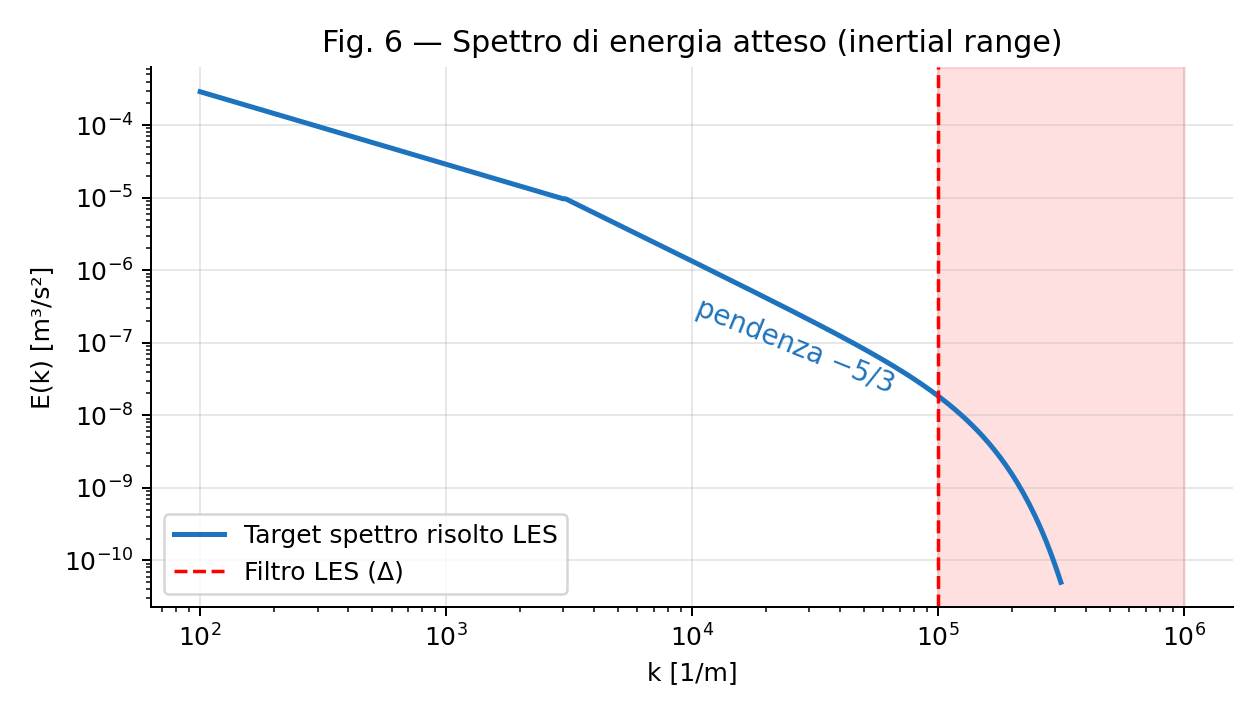
\includegraphics[width=0.88\textwidth]{fig_spectra}
  \caption{Spettro di energia turbolenta atteso dalla WRLES: range di produzione (basse frequenze), range inerziale ($-5/3$, frequenze medie), range dissipativo (alte frequenze). Le curve colorate indicano le previsioni per diversi livelli di mesh.}
  \label{fig:spectra}
\end{figure}

Lo spettro di energia turbolenta di Kolmogorov-Obukhov ha la forma:
\begin{equation}
  E(k) = C_K\,\varepsilon^{2/3}\,k^{-5/3}
  \qquad L_0^{-1} \ll k \ll \eta^{-1}
\end{equation}
dove $k$ è il numero d'onda, $C_K \approx 1.5$ è la costante di Kolmogorov e $\varepsilon$ il tasso di dissipazione. Nel dominio delle frequenze:
\begin{equation}
  S_{uu}(f) \propto f^{-5/3}
\end{equation}
tramite la relazione di Taylor (flusso gelato) $k = 2\pi f/\bar{U}$.

Per il getto in esame, la frequenza di transizione verso il range dissipativo è:
\begin{equation}
  f_\eta = \frac{\bar{U}}{2\pi\,\eta}
  = \frac{10}{2\pi \times 7\times10^{-6}}
  \approx 227\,\text{kHz}
\end{equation}
ben oltre il range di Nyquist della simulazione (20--50\,kHz). Il range inerziale atteso è molto limitato a causa del basso $Re_\lambda$.

\subsection{Indice di qualità LES di Pope}

L'indice di qualità M di Pope \cite{Pope2000} è la metrica standard per valutare la qualità di una simulazione LES:
\begin{equation}
  M(\mathbf{x}) = \frac{k_{\mathrm{ris}}}{k_{\mathrm{ris}} + k_{\mathrm{sgs}}}
\end{equation}

Il criterio di Pope richiede $M > 0.80$ in almeno l'80\% del volume. Nella pratica, per la WRLES L5:
\begin{itemize}
  \item Zone lontane da parete (bulk shear layer): $M \approx 0.90$--$0.95$ (mesh adeguata)
  \item Zone di stagnation point (impatto su chip): $M \approx 0.80$--$0.85$ (critico, da monitorare)
  \item Zone outlet (boundary numerica): $M < 0.80$ (tollerato, periferia del dominio)
\end{itemize}

L'indice M viene calcolato in SU2 includendo \ttcfg{LES\_CONST} nell'output volumetrico e post-processando con ParaView o VisIt.

\subsection{Identificazione strutture vorticose}

La visualizzazione delle strutture vorticose si effettua tramite il criterio Q (secondo invariante del tensore gradiente di velocità):
\begin{equation}
  Q = \frac{1}{2}\left(\|\boldsymbol{\Omega}\|^2 - \|\mathbf{S}\|^2\right) > 0
\end{equation}
dove $\boldsymbol{\Omega}$ e $\mathbf{S}$ sono la parte antisimmetrica (rotazione) e simmetrica (deformazione) del tensore gradiente. Le regioni con $Q > 0$ sono dominate dalla rotazione e identificano i vortici coerenti del getto.

SU2 calcola $Q$ automaticamente includendo \ttcfg{Q\_CRITERION} in \ttcfg{VOLUME\_OUTPUT}.

% ============================================================
\section{Decisioni Progettuali Aperte}
\label{sec:decisioni}
% ============================================================

Le seguenti decisioni non sono ancora state prese definitivamente e richiedono un confronto con il committente prima di avviare le simulazioni ad alto costo.

\subsection{Scelta del modello SGS: WALE vs Vreman}

Il modello WALE \cite{Nicoud1999} è scelto come default (Sezione~\ref{sec:simparams}). Un'alternativa è il modello di Vreman \cite{Vreman2004}:
\begin{equation}
  \mu_{\mathrm{sgs}}^{\mathrm{Vreman}} = \rho\,c_V\,\sqrt{\frac{B_\beta}{\alpha_{ij}\alpha_{ij}}}
  \qquad B_\beta = \beta_{11}\beta_{22}-\beta_{12}^2+\ldots
\end{equation}
Il modello di Vreman è più semplice da implementare e ha proprietà di parete simili al WALE. SU2 v8 non supporta Vreman nativamente; richiederebbe una modifica del codice o l'uso di \ttcfg{KIND\_SGS\_MODEL= DYNAMIC\_SMAGORINSKY} come alternativa dinamica.

\textbf{Decisione suggerita:} WALE come baseline; sensitivity check con Dynamic Smagorinsky se il caso principale mostra anomalie nel near-wall ($y^+ < 2$).

\subsection{Posizionamento della superficie FW-H}

La superficie di controllo FW-H deve essere posizionata in una zona dove:
\begin{enumerate}
  \item Il flusso è dominato da pressione lineare (non nonlineare)
  \item La mesh è sufficientemente fine da risolvere le onde acustiche
  \item Il dominio è chiuso (nessun attraversamento da strutture vorticose coerenti)
\end{enumerate}

\textbf{Opzione A:} superficie chiusa a $r = 0.5\,\Dcam = 10$\,mm, racchiudente la camera. \emph{Problema:} l'outlet laterale è all'interno della superficie, generando errori nell'integrazione FW-H (flusso di massa in entrata/uscita).

\textbf{Opzione B:} superficie solo sul chip (disco, $r < \Dcam/2$). Cattura solo le sorgenti dipolari di parete (dominanti a basso Ma). \emph{Vantaggio:} semplice, robusto. \emph{Svantaggio:} perde le sorgenti quadrupolari dello shear layer.

\textbf{Opzione C:} superficie conformata attorno al getto, escludendo l'outlet laterale. Più complessa da definire in Ennova ma tecnicamente corretta.

\textbf{Decisione suggerita:} Opzione B come prima verifica; Opzione C per il caso principale se le risorse di mesh lo consentono.

\subsection{Estensione del dominio per FW-H}

Il dominio computazionale attuale (camera D=20\,mm, H=3\,mm) è molto compatto. Per il calcolo acustico far-field sono possibili due approcci:

\begin{description}
  \item[Approccio A — FW-H puro:] usare il dominio attuale come near-field, applicare l'integrale FW-H su superficie di controllo e propagare al punto osservatore (r=2\,m) analiticamente. Questo è l'approccio standard e quello implementato in SU2. Funziona bene se il dominio racchiude tutte le sorgenti significative.
  \item[Approccio B — Dominio esteso:] estendere il dominio computazionale a r=50\,mm e z=-10\,mm (semispazio sotto il chip), risolvere esplicitamente la propagazione acustica nel near-field. Questo approccio è costoso (fattore 50x in volume) e richiede un solutore acustico esplicito (non il solutore incompressibile).
\end{description}

\textbf{Decisione suggerita:} Approccio A (FW-H puro), coerente con le capacità di SU2 e le risorse disponibili.

\subsection{Turbolenza di ingresso (inlet turbulence)}

Il profilo di velocità uniforme all'inlet non genera fluttuazioni di turbolenza sintetiche. In un getto reale, la turbolenza residua nell'ugello eccita più rapidamente l'instabilità di Kelvin-Helmholtz nello shear layer e accelera la transizione.

\textbf{Opzione A:} inlet deterministico (plug flow, no turbulence). Semplice, riproducibile. La transizione avviene naturalmente per instabilità numerica (noise numerico).

\textbf{Opzione B:} inlet stocastico con metodo di Klein (SU2 supporta \ttcfg{INLET\_TURBULENCE= YES} con intensità e scala della lunghezza specificate). Più realistico ma introduce parametri aggiuntivi (TI\%, $L_t$) che devono essere misurati o stimati.

\textbf{Decisione suggerita:} Opzione A per la simulazione di validazione (per confronto diretto con i dati sperimentali, dove le condizioni di inlet sono note con precisione). Opzione B per studi parametrici futuri.

% ============================================================
\section{Roadmap Temporale}
\label{sec:roadmap}
% ============================================================

\subsection{Cronoprogramma a 4 mesi}

Il programma di lavoro si sviluppa in 4 mesi (aprile--luglio 2026) secondo le fasi descritte di seguito.

\begin{table}[H]
  \centering
  \caption{Roadmap temporale a 4 mesi: attività settimanali, milestone e deliverable.}
  \label{tab:roadmap}
  \rowcolors{2}{lightblue!40}{white}
  \begin{tabularx}{\textwidth}{p{2.2cm}lX}
    \toprule
    \rowcolor{tablehead}
    \textbf{Periodo} & \textbf{HW} & \textbf{Attività e Deliverable} \\
    \midrule
    Mese\,1 Sett.\,1--2 & Laptop & Setup mesh Ennova L0--L1; config SU2 baseline; validazione topologia BC su L0. \textit{Deliverable: mesh L0 e L1 validate, RANS converge su L0.} \\
    Mese\,1 Sett.\,3--4 & Laptop & RANS SST su L1+L2+L3; calcolo GCI Celik; reportino convergenza di griglia. \textit{Deliverable: GCI < 5\% per $C_p$ chip.} \\
    Mese\,2 Sett.\,1 & Laptop & URANS SST L2 ($\Delta t = 10\mus$, 6\,000 step); FFT pressione; identificazione Strouhal. \textit{Deliverable: spettro di pressione sul chip, identificazione $\Str$.} \\
    Mese\,2 Sett.\,2--3 & Laptop/HPC & DDES SA L3 ($\Delta t = 5\mus$, 8\,000 step); verifica spettro $-5/3$ nello shear layer. \textit{Deliverable: spettro velocità con slope inerziale.} \\
    Mese\,2 Sett.\,4 & Admin & Apertura account CINECA (ISCRA-C) o AWS; deploy SU2 v8 su cluster; smoke test su L1. \\
    Mese\,3 Sett.\,1--2 & HPC & WMLES WALE L4 (256 core, 40\,ms); calcolo Pope M; primo confronto con PIV Huawei. \textit{Deliverable: campo di velocità media L4, M-index map.} \\
    Mese\,3 Sett.\,3--4 & HPC & Inizializzazione WRLES L5 da WMLES; preflush 10\,ms; avvio raccolta statistiche. \\
    Mese\,4 Sett.\,1--2 & HPC & WRLES L5 statistiche (32\,ms $= 8\,\tFT$); FW-H post-processing; SPL$(f)$ agli osservatori. \textit{Deliverable: spettro acustico far-field.} \\
    Mese\,4 Sett.\,3--4 & Post & Confronto quantitativo con misure sperimentali Huawei (PIV, hot-wire, microfono); documentazione finale; relazione tecnica. \textit{Deliverable: rapporto finale, database CFD.} \\
    \bottomrule
  \end{tabularx}
\end{table}

\subsection{Milestone principali}

\begin{enumerate}
  \item \textbf{M1 (fine Mese 1):} GCI < 5\% su quantità di interesse primarie (campo di pressione, velocità assiale). Mesh L0--L3 disponibili e validate.
  \item \textbf{M2 (fine Mese 2):} Numero di Strouhal del getto identificato e confrontato con le predizioni teoriche. Account HPC attivo e testato.
  \item \textbf{M3 (metà Mese 3):} Prima LES (WMLES L4) completata; Pope M-index $>$ 0.80 verificato in almeno 85\% del volume.
  \item \textbf{M4 (fine Mese 4):} WRLES L5 con statistiche convergenti; confronto quantitativo con dati sperimentali Huawei; relazione tecnica consegnata.
\end{enumerate}

\subsection{Rischi e mitigazioni}

\begin{description}
  \item[Rischio 1 — GCI non soddisfatto:] se la variazione tra L2 e L3 supera il 5\%, si procede comunque alla fase URANS/DDES con L3 come mesh di riferimento, documentando l'incertezza numerica.
  \item[Rischio 2 — Divergenza LES:] problemi numerici nella transizione da DDES a WMLES. Mitigazione: scendere a CFL = 0.1 per i primi 5\,000 step; verificare qualità mesh nella zona di transizione prism-tet.
  \item[Rischio 3 — Coda HPC lunga:] se la coda CINECA supera i 5 giorni lavorativi, attivare in parallelo un'istanza AWS hpc6a Spot come backup.
  \item[Rischio 4 — Memoria insufficiente su laptop:] per DDES L3 con memoria al limite, ridurre l'output volumetrico (aumentare \ttcfg{OUTPUT\_WRT\_FREQ} a 2\,000 step).
  \item[Rischio 5 — Discrepanza con esperimento:] se la WRLES mostra errori $> 20\%$ sui profili di velocità, verificare: (a) profilo di inlet (uniform plug vs parabolic), (b) modello SGS, (c) condizioni termiche.
\end{description}

% ============================================================
\section{Conclusioni}
\label{sec:conclusioni}
% ============================================================

Questo documento ha presentato il setup completo per la simulazione CFD aeroacustica del getto impingente su chip per Huawei Research Center Finland. I punti principali sono:

\begin{enumerate}
  \item \textbf{Il problema fisico} è ben caratterizzato: $\Rey = 1000$, $\Ma = 0.029$, dominio compatto di 20\,mm di diametro. Il basso numero di Reynolds implica turbolenza debolmente sviluppata, con $Re_\lambda \approx 0.87$ e range inerziale molto limitato.

  \item \textbf{L'approccio numerico} adottato (SU2 incompressibile + analogia FW-H) è appropriato per il regime di flusso. La pipeline di validazione a 6 fasi (RANS $\rightarrow$ URANS $\rightarrow$ DDES $\rightarrow$ WMLES $\rightarrow$ WRLES $\rightarrow$ FW-H) garantisce una progressione controllata nell'uso delle risorse computazionali.

  \item \textbf{Il laptop del committente} (Ryzen 9 AI 370 HX) è adeguato per le fasi RANS e URANS (fino a $\approx 3$\,M celle, qualche giorno di calcolo). Le simulazioni LES richiedono obbligatoriamente HPC.

  \item \textbf{Il costo computazionale} del percorso completo fino alla WRLES L5 è dell'ordine di \texteuro 1\,600 su CINECA accademico o \$2\,700 su AWS Spot. Il costo è dominato dalla WRLES L5 (12\,M celle, 100\,000 step), che assorbe $\approx 75\%$ del budget.

  \item \textbf{La roadmap a 4 mesi} è realistica, a condizione di: (a) avere la mesh L0--L1 disponibile entro la prima settimana, (b) aprire l'account CINECA entro la fine del Mese 2, (c) non incorrere in problemi di convergenza LES che richiedano modifiche alla mesh.

  \item \textbf{Le decisioni progettuali aperte} (modello SGS, posizionamento FW-H, turbolenza di ingresso) sono descritte nella Sezione~\ref{sec:decisioni}. Le scelte di default raccomandate sono conservative e adatte alla fase di validazione iniziale.
\end{enumerate}

La commessa di validazione descritta in questo documento costituisce la base scientifica necessaria per le fasi successive: ottimizzazione della geometria, studio della configurazione con mesh cubica e, in prospettiva, design assistito da CFD ad alta fedeltà per chip di prossima generazione.

% ============================================================
% RIFERIMENTI
% ============================================================
\newpage
\begin{thebibliography}{99}
\small

\bibitem{Pope2000}
  Pope, S.B. (2000).
  \textit{Turbulent Flows}.
  Cambridge University Press.

\bibitem{Celik2008}
  Celik, I.B., Ghia, U., Roache, P.J., Freitas, C.J., Coleman, H., Raad, P.E. (2008).
  Procedure for Estimation and Reporting of Uncertainty Due to Discretization in CFD Applications.
  \textit{Journal of Fluids Engineering}, 130(7), 078001.

\bibitem{Nicoud1999}
  Nicoud, F. \& Ducros, F. (1999).
  Subgrid-scale stress modelling based on the square of the velocity gradient tensor.
  \textit{Flow, Turbulence and Combustion}, 62(3), 183--200.

\bibitem{Vreman2004}
  Vreman, A.W. (2004).
  An eddy-viscosity subgrid-scale model for turbulent shear flow:
  algebraic theory and applications.
  \textit{Physics of Fluids}, 16(10), 3670--3681.

\bibitem{Shur2005}
  Shur, M.L., Spalart, P.R. \& Strelets, M.Kh. (2005).
  Noise prediction for increasingly complex jets. Part I: Methods and tests.
  \textit{International Journal of Aeroacoustics}, 4(3--4), 213--266.

\bibitem{Hadziabdic2008}
  Hadziabdic, M. \& Hanjalic, K. (2008).
  Vortical structures and heat transfer in a round impinging jet.
  \textit{Journal of Fluid Mechanics}, 596, 221--260.

\bibitem{Dairay2015}
  Dairay, T., Fortune, V., Lamballais, E. \& Brizzi, L.-E. (2015).
  Direct numerical simulation of a turbulent jet impinging on a heated wall.
  \textit{Journal of Fluid Mechanics}, 764, 362--394.

\bibitem{Economon2016}
  Economon, T.D., Palacios, F., Copeland, S.R., Lukaczyk, T.W. \& Alonso, J.J. (2016).
  SU2: An Open-Source Suite for Multiphysics Design and Analysis.
  \textit{AIAA Journal}, 54(3), 828--846.

\bibitem{Zhou2018}
  Zhou, B.Y., Albring, T., Gauger, N.R., Economon, T.D. \& Alonso, J.J. (2018).
  Efficient Parallel Adjoint Approach for Aeroacoustic Prediction and Optimization in SU2.
  \textit{AIAA Paper 2018--3530}.

\bibitem{Viswanathan2004}
  Viswanathan, K. (2004).
  Aeroacoustics of hot jets.
  \textit{Journal of Fluid Mechanics}, 516, 39--82.

\bibitem{FfowcsHawkings1969}
  Ffowcs-Williams, J.E. \& Hawkings, D.L. (1969).
  Sound generation by turbulence and surfaces in arbitrary motion.
  \textit{Philosophical Transactions of the Royal Society of London A},
  264(1151), 321--342.

\bibitem{Spalart2006}
  Spalart, P.R., Deck, S., Shur, M.L., Squires, K.D., Strelets, M.Kh. \& Travin, A. (2006).
  A new version of detached-eddy simulation, resistant to ambiguous grid densities.
  \textit{Theoretical and Computational Fluid Dynamics}, 20(3), 181--195.

\end{thebibliography}

\end{document}
